\section{Introduction}\label{introduction}

Quantitative mass spectrometry based spatial proteomics involves
elaborate, expensive and time consuming experimental procedures and
considerable effort is invested in the generation of such data. Multiple
research groups have described a variety of approaches to establish high
quality proteome-wide datasets. However, data analysis is as critical as
data production for reliable and insightful biological interpretation.
Here, we walk the reader through a typical pipeline for the analysis of
such data using several Bioconductor packages for the R statistical
programming environment.

The main package to analyse protein localisation data is
\texttt{r Biocpkg("pRoloc")}, which offers a set of dedicated functions
for the analysis of such data.
\emph{\href{http://bioconductor.org/packages/pRoloc}{pRoloc}} itself
relies on \texttt{r Biocpkg("MSnbase")} to manipulate and process
quantitative proteomics data. Many other packages are used by
\emph{\href{http://bioconductor.org/packages/pRoloc}{pRoloc}} for
clustering, classification and visualisation.

In this workflow, we will describe how to prepare the spatial proteomics
data starting from a spreadsheet containing quantitative mass
spectrometry data. We will focus on a recent pluripotent mouse embryonic
stem cells experiment {[}@hyper{]}. Additional annotated and
pre-formatted datasets from various species are readily available in the
\emph{\href{http://bioconductor.org/packages/pRolocdata}{pRolocdata}}
package.

Installation of Bioconductor package is documented in details on the
\href{http://bioconductor.org/install/\#install-bioconductor-packages}{Bioconductor
installation help page}. This procedure is also applicable to any
packages, from \href{https://cran.r-project.org/}{CRAN} as well as
GitHub. Once a package has been installed, it needs to be loaded for its
functionality to become available in the R session; this is done with
the \texttt{library} function e.g. to load the
\emph{\href{http://bioconductor.org/packages/pRoloc}{pRoloc}} one would
type \texttt{library("pRoloc")} after installation.

If you have questions about this workflow in particular, or about other
Bioconductor packages in general, they are best asked on the
\href{https://support.bioconductor.org/}{Bioconductor support site}
following the
\href{http://www.bioconductor.org/help/support/posting-guide/}{posting
guidelines}. Questions can be tagged with specific package names or
keywords. For more general information about mass spectrometry and
proteomics, the readers are invited to read the
\emph{\href{http://bioconductor.org/packages/RforProteomics}{RforProteomics}}
package vignettes and associated papers {[}@Gatto:2014;@Gatto2015{]}.

\section{Reading and processing spatial proteomics
data}\label{reading-and-processing-spatial-proteomics-data}

\subsection{The use-case: predicting sub-cellular localisation in
pluripotent embryonic mouse stem
cells}\label{the-use-case-predicting-sub-cellular-localisation-in-pluripotent-embryonic-mouse-stem-cells}

As a use-case, we analyse a recent high-throughput spatial proteomics
dataset from pluripotent mouse embryonic stem cells (E14TG2a)
{[}@hyper{]}. The data was generated using hyperplexed LOPIT
(hyperLOPIT), a state-of-the-art method relying on improved sub-cellular
fractionation and more accurate quantitation, leading to more reliable
classification of protein localisation across the whole sub-cellular
space. The method uses an elaborate sub-cellular fractionation scheme,
enabled by the use of Tandem Mass Tag (TMT) {[}Thompson:2003{]} 10-plex
and application of the MS data acquisition technique named synchronous
precursor selection MS\textsuperscript{3} (SPS-MS\textsuperscript{3})
{[}@McAlister:2014{]}, for TMT quantification with high accuracy and
precision. Three biological replicates were generated from the E14TG2a
experiment, the first was to target low density fractions and the second
and third were to emphasis separation of the denser organelles. The
intersect of replicates 1 and 2 was treated as a 20-plex dataset for the
analysis. As discussed in the manuscript {[}@hyper{]} as it has been
shown that combining replicates across from different gradients can
increase spatial resolution {[}@Trotter:2010{]}. The combination of
replicates resulted in 5032 proteins common in both experiments.

These, as well as many other data are directly available as properly
structured and annotated computational object from the
\emph{\href{http://bioconductor.org/packages/pRolocdata}{pRolocdata}}
experiment package. In this workflow, we will start with a description
of how to generate these ad hoc objects starting from an arbitrary
spreadsheets, as produced by many popular third-party applications.

While we focus here on a LOPIT-type dataset, these analyses are relevant
for any quantitative spatial proteomics data, irrespective of the
fractionation or quantitation (i.e.~labelled or label-free) methods.

\subsection{The infrastructure:
\emph{\href{http://bioconductor.org/packages/pRoloc}{pRoloc}} and
\emph{\href{http://bioconductor.org/packages/MSnbase}{MSnbase}} in
Bioconductor}\label{the-infrastructure-proloc-and-msnbase-in-bioconductor}

To make use of the full functionality of the
\emph{\href{http://bioconductor.org/packages/pRoloc}{pRoloc}} software
one needs to import their data into R and prepare them as an
\texttt{MSnSet}. The \texttt{MSnSet} is a dedicated data structure for
the efficient manipulation and processing of mass spectrometry and
proteomics data in R. Figure 1 illustrates a simplified view of the
\texttt{MSnSet} structure; there exists 3 key sub-parts (termed slots)
to such a data object: (1) the \texttt{exprs} slot for storing the
quantitation data, (2) the \texttt{fData} slot for storing the feature
meta-data, and finally (3) the \texttt{pData} slot for storing the
sample meta-data.

\begin{figure}[htbp]
\centering
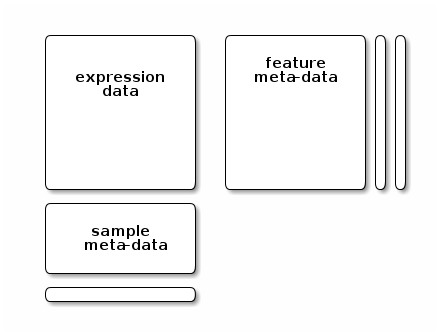
\includegraphics{./Figures/msnset.png}
\caption{Simplified representation of the \texttt{MSnSet} data structure
(reproduced with permission from the
\emph{\href{http://bioconductor.org/packages/MSnbase}{MSnbase}}
vignette)}
\end{figure}

\subsection{Importing data}\label{importing-data}

There are a number of ways to import quantitation data and create an
\texttt{MSnSet} instance. All methods are described in the
\emph{\href{http://bioconductor.org/packages/MSnbase}{MSnbase}}
\href{http://bioconductor.org/packages/release/bioc/vignettes/MSnbase/inst/doc/MSnbase-io.pdf}{input/output
capabilities vignette}. One suggested simple method is to use the
function \texttt{readMSnSet2} in
\emph{\href{http://bioconductor.org/packages/MSnbase}{MSnbase}}. The
function takes a single spreadsheet as input and extracts the columns
containing the quantitation data, as identified by the argument
\texttt{ecol}, to create the expression data, while the other columns in
the spreadsheet are appended to the feature meta-data slot. By example,
in the code chunk below we read in the \texttt{csv} spreadsheet
containing the quantitation data from the intersect of replicates 1 and
2 of the mouse map {[}@hyper{]}, using the \texttt{readMSnSet2}
function. The data is as available online with the manuscript (see tab 2
of the \texttt{xlsx} supplementary data set 1 in {[}@hyper{]}, which
should be exported as a text-based spreadsheet). It is also available as
a \texttt{csv} in the Bioconductor \texttt{r Biocexptpkg("pRolocdata")}
data package.

To use the \texttt{readMSnSet2} function, as a minimum one must specify
the file path to the data and which columns of the spreadsheet contain
quantitation data. The \texttt{getEcols} function exists to help users
identify which columns of the spreadsheet contain the quantitation data.
In the last line of the code chunk below, we print the file name (not
the full path, which will vary from computer to computer).

\begin{Shaded}
\begin{Highlighting}[]
\KeywordTok{library}\NormalTok{(}\StringTok{"MSnbase"}\NormalTok{)}
\NormalTok{extdatadir <-}\StringTok{ }\KeywordTok{system.file}\NormalTok{(}\StringTok{"extdata"}\NormalTok{, }\DataTypeTok{package =} \StringTok{"pRolocdata"}\NormalTok{)}
\NormalTok{csvfile <-}\StringTok{ }\KeywordTok{dir}\NormalTok{(extdatadir, }\DataTypeTok{full.names =} \OtherTok{TRUE}\NormalTok{,}
          \DataTypeTok{pattern =} \StringTok{"hyperLOPIT-SIData-ms3-rep12-intersect.csv"}\NormalTok{)}
\KeywordTok{basename}\NormalTok{(csvfile)}
\end{Highlighting}
\end{Shaded}

\begin{verbatim}
## [1] "hyperLOPIT-SIData-ms3-rep12-intersect.csv.gz"
\end{verbatim}

Note that the file is compressed (as indicated by the \texttt{gz}, for
\texttt{gzip}, extension), and will be decompressed on-the-fly when read
into R later on.

The spreadsheet that was deposited by the authors contains two headers,
with the second header containing information about where the
quantitation data is stored.

\begin{figure}[htbp]
\centering
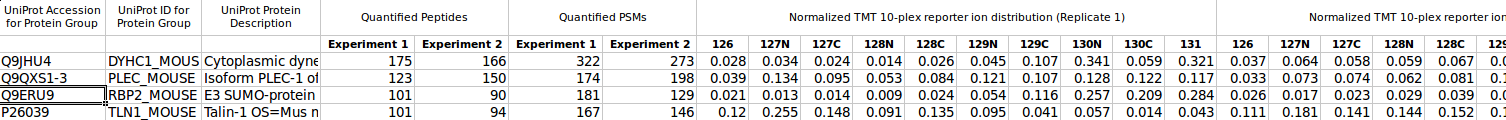
\includegraphics{./Figures/spreadsheet-screenshot.png}
\caption{A screenshot of the data in the spreadsheet.}
\end{figure}

We can display the names of the second header by calling the
\texttt{getEcols} function with the argument \texttt{n = 2} (the default
value is \texttt{n = 1}), to specify that we wish to display the column
names of the second line.

\begin{Shaded}
\begin{Highlighting}[]
\KeywordTok{getEcols}\NormalTok{(csvfile, }\DataTypeTok{split =} \StringTok{","}\NormalTok{, }\DataTypeTok{n =} \DecValTok{2}\NormalTok{)}
\end{Highlighting}
\end{Shaded}

\begin{verbatim}
##  [1] ""                                 
##  [2] ""                                 
##  [3] ""                                 
##  [4] "Experiment 1"                     
##  [5] "Experiment 2"                     
##  [6] "Experiment 1"                     
##  [7] "Experiment 2"                     
##  [8] "126"                              
##  [9] "127N"                             
## [10] "127C"                             
## [11] "128N"                             
## [12] "128C"                             
## [13] "129N"                             
## [14] "129C"                             
## [15] "130N"                             
## [16] "130C"                             
## [17] "131"                              
## [18] "126"                              
## [19] "127N"                             
## [20] "127C"                             
## [21] "128N"                             
## [22] "128C"                             
## [23] "129N"                             
## [24] "129C"                             
## [25] "130N"                             
## [26] "130C"                             
## [27] "131"                              
## [28] "phenoDisco Input"                 
## [29] "phenoDisco Output"                
## [30] "Curated phenoDisco Output"        
## [31] "SVM marker set"                   
## [32] "SVM classification"               
## [33] "SVM score"                        
## [34] "SVM classification (top quartile)"
## [35] "Final Localization Assignment"    
## [36] "First localization evidence?"     
## [37] "Curated Organelles"               
## [38] "Cytoskeletal Components"          
## [39] "Trafficking Proteins"             
## [40] "Protein Complexes"                
## [41] "Signaling Cascades"               
## [42] "Oct4 Interactome"                 
## [43] "Nanog Interactome"                
## [44] "Sox2 Interactome"                 
## [45] "Cell Surface Proteins"
\end{verbatim}

It is now easy for one to identify that the quantitation data,
corresponding to the 10 TMT isobaric tags, is located in columns 8 to
27. We now have the two mandatory arguments to \texttt{readMSnSet2},
namely the file name (stored in the \texttt{csvfile} variable) and the
quantitation column indices. In addition to these, it is also possible
to pass the optional argument \texttt{fnames} to indicate which column
to use as the labels by which to identify each protein in the sample.
Here, we use \texttt{fnames = 1} to use the UniProt identifiers
contained in the first (unnamed) column of the spreadsheet. We also need
to specify to skip the first line of the file (for the same reason that
we used \texttt{n = 2} in \texttt{getEcols} above) to read the
\texttt{csv} data and convert it to an \texttt{MSnSet} object, named
\texttt{hl} (for hyperLOPIT).

\begin{Shaded}
\begin{Highlighting}[]
\NormalTok{hl <-}\StringTok{ }\KeywordTok{readMSnSet2}\NormalTok{(csvfile, }\DataTypeTok{ecol =} \DecValTok{8}\NormalTok{:}\DecValTok{27}\NormalTok{, }\DataTypeTok{fnames =} \DecValTok{1}\NormalTok{, }\DataTypeTok{skip =} \DecValTok{1}\NormalTok{)}
\end{Highlighting}
\end{Shaded}

Below, we display a short summary of the data. The data contains 5032
proteins/features common across the 2 biological replicates for the
respective 2 x 10-plex reporter tags (20 columns/samples), along with
associated feature meta-data such as protein markers, protein
description, number of quantified peptides etc (see below).

\begin{Shaded}
\begin{Highlighting}[]
\NormalTok{hl}
\end{Highlighting}
\end{Shaded}

\begin{verbatim}
## MSnSet (storageMode: lockedEnvironment)
## assayData: 5032 features, 20 samples 
##   element names: exprs 
## protocolData: none
## phenoData: none
## featureData
##   featureNames: Q9JHU4 Q9QXS1-3 ... Q9Z2R6 (5032 total)
##   fvarLabels: X X.1 ... Cell.Surface.Proteins (25 total)
##   fvarMetadata: labelDescription
## experimentData: use 'experimentData(object)'
## Annotation:  
## - - - Processing information - - -
##  MSnbase version: 1.99.2
\end{verbatim}

Below, we examine the quantitative information for first 5 proteins. It
is also possible to access specific rows and columns by naming the
proteins and TMT tag channels of interest.

\begin{Shaded}
\begin{Highlighting}[]
\KeywordTok{exprs}\NormalTok{(hl)[}\DecValTok{1}\NormalTok{:}\DecValTok{5}\NormalTok{, ]}
\end{Highlighting}
\end{Shaded}

\begin{verbatim}
##           X126 X127N X127C X128N X128C X129N X129C X130N X130C  X131
## Q9JHU4   0.028 0.034 0.024 0.014 0.026 0.045 0.107 0.341 0.059 0.321
## Q9QXS1-3 0.039 0.134 0.095 0.053 0.084 0.121 0.107 0.128 0.122 0.117
## Q9ERU9   0.021 0.013 0.014 0.009 0.024 0.054 0.116 0.257 0.209 0.284
## P26039   0.120 0.255 0.148 0.091 0.135 0.095 0.041 0.057 0.014 0.043
## Q8BTM8   0.055 0.139 0.078 0.050 0.077 0.098 0.093 0.171 0.079 0.160
##          X126.1 X127N.1 X127C.1 X128N.1 X128C.1 X129N.1 X129C.1 X130N.1
## Q9JHU4    0.037   0.064   0.058   0.059   0.067   0.078   0.140   0.208
## Q9QXS1-3  0.033   0.073   0.074   0.062   0.081   0.142   0.190   0.069
## Q9ERU9    0.026   0.017   0.023   0.029   0.039   0.071   0.105   0.171
## P26039    0.111   0.181   0.141   0.144   0.152   0.119   0.075   0.028
## Q8BTM8    0.062   0.108   0.091   0.086   0.099   0.111   0.117   0.095
##          X130C.1 X131.1
## Q9JHU4     0.141  0.147
## Q9QXS1-3   0.151  0.125
## Q9ERU9     0.304  0.215
## P26039     0.017  0.033
## Q8BTM8     0.144  0.087
\end{verbatim}

\begin{Shaded}
\begin{Highlighting}[]
\KeywordTok{exprs}\NormalTok{(hl)[}\KeywordTok{c}\NormalTok{(}\StringTok{"Q9ERU9"}\NormalTok{, }\StringTok{"Q9Z2R6"}\NormalTok{), }\KeywordTok{c}\NormalTok{(}\StringTok{"X126"}\NormalTok{, }\StringTok{"X131.1"}\NormalTok{)]}
\end{Highlighting}
\end{Shaded}

\begin{verbatim}
##         X126 X131.1
## Q9ERU9 0.021  0.215
## Q9Z2R6 0.563  0.000
\end{verbatim}

The feature meta-data is stored in the \texttt{fData} slot and can be
accessed by \texttt{fData(hl)}. When using \texttt{readMSnSet2},
automatically, everything that is not defined as quantitation data by
\texttt{ecol} or the feature names by \texttt{fnames} is deposited to
the \texttt{fData} slot.

We see the \texttt{fData} contains 25 columns describing information
such as the number of peptides, associated markers, machine learning
results etc. To identify the feature variable names we can use the
function \texttt{fvarLabels}. We see that the first 6 feature variable
names contain non-discriminatory label names, so we relabel them to help
us identify what feature data information is stored in the associated
columns.

\begin{Shaded}
\begin{Highlighting}[]
\KeywordTok{fvarLabels}\NormalTok{(hl)}
\end{Highlighting}
\end{Shaded}

\begin{verbatim}
##  [1] "X"                                
##  [2] "X.1"                              
##  [3] "X.2"                              
##  [4] "Experiment.1"                     
##  [5] "Experiment.2"                     
##  [6] "Experiment.1.1"                   
##  [7] "Experiment.2.1"                   
##  [8] "phenoDisco.Input"                 
##  [9] "phenoDisco.Output"                
## [10] "Curated.phenoDisco.Output"        
## [11] "SVM.marker.set"                   
## [12] "SVM.classification"               
## [13] "SVM.score"                        
## [14] "SVM.classification..top.quartile."
## [15] "Final.Localization.Assignment"    
## [16] "First.localization.evidence."     
## [17] "Curated.Organelles"               
## [18] "Cytoskeletal.Components"          
## [19] "Trafficking.Proteins"             
## [20] "Protein.Complexes"                
## [21] "Signaling.Cascades"               
## [22] "Oct4.Interactome"                 
## [23] "Nanog.Interactome"                
## [24] "Sox2.Interactome"                 
## [25] "Cell.Surface.Proteins"
\end{verbatim}

\begin{Shaded}
\begin{Highlighting}[]
\KeywordTok{fvarLabels}\NormalTok{(hl)[}\DecValTok{1}\NormalTok{:}\DecValTok{3}\NormalTok{] <-}\StringTok{ }\KeywordTok{c}\NormalTok{(}\StringTok{"uniprot.accession"}\NormalTok{, }\StringTok{"uniprot.id"}\NormalTok{, }\StringTok{"description"}\NormalTok{)}
\KeywordTok{fvarLabels}\NormalTok{(hl)[}\DecValTok{4}\NormalTok{:}\DecValTok{6}\NormalTok{] <-}\StringTok{ }\KeywordTok{paste0}\NormalTok{(}\StringTok{"peptides.expt"}\NormalTok{, }\DecValTok{1}\NormalTok{:}\DecValTok{3}\NormalTok{)}
\KeywordTok{fData}\NormalTok{(hl)[}\DecValTok{1}\NormalTok{:}\DecValTok{4}\NormalTok{, }\DecValTok{1}\NormalTok{:}\DecValTok{6}\NormalTok{]}
\end{Highlighting}
\end{Shaded}

\begin{verbatim}
##          uniprot.accession  uniprot.id
## Q9JHU4              Q9JHU4 DYHC1_MOUSE
## Q9QXS1-3          Q9QXS1-3  PLEC_MOUSE
## Q9ERU9              Q9ERU9  RBP2_MOUSE
## P26039              P26039  TLN1_MOUSE
##                                                                                                                                 description
## Q9JHU4                                              Cytoplasmic dynein 1 heavy chain 1 OS=Mus musculus GN=Dync1h1 PE=1 SV=2 - [DYHC1_MOUSE]
## Q9QXS1-3 Isoform PLEC-1 of Plectin OS=Mus musculus GN=Plec - [PLEC_MOUSE]|Isoform PLEC-1A of Plectin OS=Mus musculus GN=Plec - [PLEC_MOUSE]
## Q9ERU9                                                     E3 SUMO-protein ligase RanBP2 OS=Mus musculus GN=Ranbp2 PE=1 SV=2 - [RBP2_MOUSE]
## P26039                                                                             Talin-1 OS=Mus musculus GN=Tln1 PE=1 SV=2 - [TLN1_MOUSE]
##          peptides.expt1 peptides.expt2 peptides.expt3
## Q9JHU4              175            166            322
## Q9QXS1-3            123            150            174
## Q9ERU9              101             90            181
## P26039              101             94            167
\end{verbatim}

Note that when using the simple \texttt{readMSnSet2} procedure, the
\texttt{pData} slot which is used to store information about the
samples/channels is kept empty. It is advised to annotate the channels
as well. Below, we annotate the replicate from which the profiles
originate and the TMT tag (extracted from the sample/channel names).

\begin{Shaded}
\begin{Highlighting}[]
\KeywordTok{pData}\NormalTok{(hl)$Replicate <-}\StringTok{ }\KeywordTok{rep}\NormalTok{(}\DecValTok{1}\NormalTok{:}\DecValTok{2}\NormalTok{, }\DataTypeTok{each =} \DecValTok{10}\NormalTok{)}
\KeywordTok{pData}\NormalTok{(hl)$Tag <-}\StringTok{ }\KeywordTok{sub}\NormalTok{(}\StringTok{"}\CharTok{\textbackslash{}\textbackslash{}}\StringTok{.1$"}\NormalTok{, }\StringTok{""}\NormalTok{, }\KeywordTok{sub}\NormalTok{(}\StringTok{"^X"}\NormalTok{, }\StringTok{""}\NormalTok{, }\KeywordTok{sampleNames}\NormalTok{(hl)))}
\KeywordTok{pData}\NormalTok{(hl)}
\end{Highlighting}
\end{Shaded}

\begin{verbatim}
##         Replicate  Tag
## X126            1  126
## X127N           1 127N
## X127C           1 127C
## X128N           1 128N
## X128C           1 128C
## X129N           1 129N
## X129C           1 129C
## X130N           1 130N
## X130C           1 130C
## X131            1  131
## X126.1          2  126
## X127N.1         2 127N
## X127C.1         2 127C
## X128N.1         2 128N
## X128C.1         2 128C
## X129N.1         2 129N
## X129C.1         2 129C
## X130N.1         2 130N
## X130C.1         2 130C
## X131.1          2  131
\end{verbatim}

Throughout this workflow we refer to the different columns that are
found in the \texttt{exprs} (expression data) slot as channels (short
for TMT channels). In the frame of LOPIT and hyperLOPIT these channels
consititue the relative abundance of each protein (along the rows) in
the channel of interest. Each TMT channel originates from fractions
collected from the density gradient, or a set of pooled fractions or may
be a sample originating from an alternative preparation e.g.~such as
from the chromatin enrichment performed in Christoforou et al
{[}@hyper{]}. Information about which gradient fractions were used for
which tag should also be stored in the sample meta-data \texttt{pData}
slot.

The sample meta-data that is distributed with the
\emph{\href{http://bioconductor.org/packages/pRolocdata}{pRolocdata}}
package for Christoforou's hyperLOPIT experiment and (as above) the
quantitation data file, are located in the \texttt{extdata} in the
\emph{\href{http://bioconductor.org/packages/pRolocdata}{pRolocdata}}
package on the hard drive.

In the code chunk below we again use the \texttt{dir} function to locate
the filepath to the meta-data \texttt{csv} file and then read it into R
using \texttt{read.csv}. We then append the meta-data to the
\texttt{pData} slot. Information about the gradient fractions used and
the associated subcellular fraction densities in \% w/v Iodixanol for
each replicate are stored here.

\begin{Shaded}
\begin{Highlighting}[]
\NormalTok{expinfo <-}\StringTok{ }\KeywordTok{dir}\NormalTok{(extdatadir, }\DataTypeTok{full.names =} \OtherTok{TRUE}\NormalTok{,}
               \DataTypeTok{pattern =} \StringTok{"hyperLOPIT-SIData-fraction-info.csv"}\NormalTok{)}

\NormalTok{fracinfo <-}\StringTok{ }\KeywordTok{read.csv}\NormalTok{(expinfo, }\DataTypeTok{row.names=}\DecValTok{1}\NormalTok{, }\DataTypeTok{skip =} \DecValTok{2}\NormalTok{, }
                     \DataTypeTok{header =} \OtherTok{FALSE}\NormalTok{, }\DataTypeTok{stringsAsFactors =} \OtherTok{FALSE}\NormalTok{)}

\KeywordTok{pData}\NormalTok{(hl)$Gradient.Fraction <-}\StringTok{ }\KeywordTok{c}\NormalTok{(fracinfo[, }\DecValTok{1}\NormalTok{], fracinfo[, }\DecValTok{2}\NormalTok{])}
\KeywordTok{pData}\NormalTok{(hl)$Iodixonal.Density <-}\StringTok{ }\KeywordTok{c}\NormalTok{(fracinfo[, }\DecValTok{4}\NormalTok{], fracinfo[, }\DecValTok{5}\NormalTok{])}
\KeywordTok{pData}\NormalTok{(hl)}
\end{Highlighting}
\end{Shaded}

\begin{verbatim}
##         Replicate  Tag Gradient.Fraction Iodixonal.Density
## X126            1  126           Cytosol               0.0
## X127N           1 127N   1 to 6 (pooled)               6.0
## X127C           1 127C   8 to 9 (pooled)              11.0
## X128N           1 128N 10 to 11 (pooled)              13.3
## X128C           1 128C                12              14.6
## X129N           1 129N                14              17.4
## X129C           1 129C                16              20.1
## X130N           1 130N                18              26.8
## X130C           1 130C         Chromatin                NA
## X131            1  131                19              34.5
## X126.1          2  126           Cytosol               0.0
## X127N.1         2 127N   1 to 6 (pooled)               5.2
## X127C.1         2 127C   7 to 9 (pooled)              10.0
## X128N.1         2 128N 10 to 11 (pooled)              12.5
## X128C.1         2 128C                12              14.0
## X129N.1         2 129N 14 to 15 (pooled)              17.3
## X129C.1         2 129C                17              20.9
## X130N.1         2 130N 18 to 19 (pooled)              24.7
## X130C.1         2 130C         Chromatin                NA
## X131.1          2  131                20              31.9
\end{verbatim}

\subsection{Data processing}\label{data-processing}

\subsubsection{Normalisation}\label{normalisation}

There are two aspects related to data normalisation that are relevant to
spatial proteomics data processing. The first one focuses on reducing
purely technical variation between channels without affecting biological
variability (i.e.~the shape of the quantitative profiles). This
normalisation will depend on the underlying quantitative technology and
the experimental design, and will not be addressed in this workflow. The
second aspect, and more specific to spatial proteomics data, is scaling
all the organelle-specific profiles into a same intensity interval
(typically 0 and 1) by, for example, diving each intensity by the sum of
the intensities for that quantitative feature. This is not necessary in
this example as the intensities for each replicate have already been
re-scaled to 1 in Proteome Discoverer. However, if one wanted to do this
they would execute the \texttt{normalise} function as demonstrated in
the below code chunk.

\begin{Shaded}
\begin{Highlighting}[]
\NormalTok{hl <-}\StringTok{ }\KeywordTok{normalise}\NormalTok{(hl, }\DataTypeTok{method =} \StringTok{"sum"}\NormalTok{) }
\end{Highlighting}
\end{Shaded}

This transformation of the data assures to cancel the effect of the
absolute intensities of the quantitative features along the rows, to
focus subsequent analyses on the relative profiles along the
sub-cellular channels.

The same \texttt{normalise} function (or \texttt{normalize}, both
spellings are supported) can also be applied in the first case described
above. Different normalisation methods such as mean or median scaling,
variance stabilisation or quantile normalisation, to cite a few, can be
applied to accomodation different needs.

As previously mentioned, before combination, the two replicates in the
\texttt{hl} data that we read into R were separately normalised by sum
(i.e.~to 1) across the 10 channels for each replicate respectively. We
can verify this by summing each rows for each replicate:

\begin{Shaded}
\begin{Highlighting}[]
\KeywordTok{summary}\NormalTok{(}\KeywordTok{rowSums}\NormalTok{(}\KeywordTok{exprs}\NormalTok{(hl[, hl$replicate ==}\StringTok{ }\DecValTok{1}\NormalTok{])))}
\end{Highlighting}
\end{Shaded}

\begin{verbatim}
##    Min. 1st Qu.  Median    Mean 3rd Qu.    Max. 
##       0       0       0       0       0       0
\end{verbatim}

\begin{Shaded}
\begin{Highlighting}[]
\KeywordTok{summary}\NormalTok{(}\KeywordTok{rowSums}\NormalTok{(}\KeywordTok{exprs}\NormalTok{(hl[, hl$replicate ==}\StringTok{ }\DecValTok{2}\NormalTok{])))}
\end{Highlighting}
\end{Shaded}

\begin{verbatim}
##    Min. 1st Qu.  Median    Mean 3rd Qu.    Max. 
##       0       0       0       0       0       0
\end{verbatim}

We see that some features do not add up exactly to 1 due to rounding
errors after exporting to intermediate files. These small deviations do
not bear any consequences here.

\subsubsection{Combining acquisitions}\label{combining-acquisitions}

The spreadsheet that was used to create the \texttt{hl} MSnSet included
the two replicates within one .csv file. We also provide individual
replicates in the
\emph{\href{http://bioconductor.org/packages/pRolocdata}{pRolocdata}}
package. Below, we show how to combine \texttt{MSnSet} objects and,
subsequently, how to filter and handle missing values. We start by
loading the \texttt{r Biocexptpkg("pRolocdata")} package and the
equivalent replicates using the \texttt{data} function.

\begin{Shaded}
\begin{Highlighting}[]
\KeywordTok{library}\NormalTok{(}\StringTok{"pRolocdata"}\NormalTok{)}
\KeywordTok{data}\NormalTok{(hyperLOPIT2015ms3r1)}
\KeywordTok{data}\NormalTok{(hyperLOPIT2015ms3r2)}
\end{Highlighting}
\end{Shaded}

At the R prompt, typing

\begin{Shaded}
\begin{Highlighting}[]
\KeywordTok{pRolocdata}\NormalTok{()}
\end{Highlighting}
\end{Shaded}

will list the 54 datasets that are available in
\emph{\href{http://bioconductor.org/packages/pRolocdata}{pRolocdata}}.

Combining data is performed with the \texttt{combine} function. This
function will inspect the feature and sample names to identify how to
combine the data. As we want our replicates to be combined along the
columns (same proteins, different sets of channels), we need to assure
that the respective sample names differ so they can be identified from
one another. The function \texttt{updateSampleNames} can be used do
this.

\begin{Shaded}
\begin{Highlighting}[]
\KeywordTok{identical}\NormalTok{(}\KeywordTok{sampleNames}\NormalTok{(hyperLOPIT2015ms3r1), }\KeywordTok{sampleNames}\NormalTok{(hyperLOPIT2015ms3r2))}
\end{Highlighting}
\end{Shaded}

\begin{verbatim}
## [1] TRUE
\end{verbatim}

\begin{Shaded}
\begin{Highlighting}[]
\NormalTok{hyperLOPIT2015ms3r1 <-}\StringTok{ }\KeywordTok{updateSampleNames}\NormalTok{(hyperLOPIT2015ms3r1, }\DecValTok{1}\NormalTok{)}
\NormalTok{hyperLOPIT2015ms3r2 <-}\StringTok{ }\KeywordTok{updateSampleNames}\NormalTok{(hyperLOPIT2015ms3r2, }\DecValTok{2}\NormalTok{)}
\KeywordTok{sampleNames}\NormalTok{(hyperLOPIT2015ms3r1)}
\end{Highlighting}
\end{Shaded}

\begin{verbatim}
##  [1] "X126.1"  "X127N.1" "X127C.1" "X128N.1" "X128C.1" "X129N.1" "X129C.1"
##  [8] "X130N.1" "X130C.1" "X131.1"
\end{verbatim}

\begin{Shaded}
\begin{Highlighting}[]
\KeywordTok{sampleNames}\NormalTok{(hyperLOPIT2015ms3r2)}
\end{Highlighting}
\end{Shaded}

\begin{verbatim}
##  [1] "X126.2"  "X127N.2" "X127C.2" "X128N.2" "X128C.2" "X129N.2" "X129C.2"
##  [8] "X130N.2" "X130C.2" "X131.2"
\end{verbatim}

In addition, to matching names, the content of the feature metadata for
identical feature annotations must match exactly across the data to be
combined. In particular for these data, we expect the same proteins in
each replicates to be annotated with the same UniProt entry names and
descriptions, but not with the same coverage of number of peptides or
peptide-spectrum matches (PSMs).

\begin{Shaded}
\begin{Highlighting}[]
\KeywordTok{fvarLabels}\NormalTok{(hyperLOPIT2015ms3r1)}
\end{Highlighting}
\end{Shaded}

\begin{verbatim}
## [1] "EntryName"          "ProteinDescription" "Peptides"          
## [4] "PSMs"               "ProteinCoverage"    "markers"
\end{verbatim}

\begin{Shaded}
\begin{Highlighting}[]
\KeywordTok{fvarLabels}\NormalTok{(hyperLOPIT2015ms3r2)}
\end{Highlighting}
\end{Shaded}

\begin{verbatim}
## [1] "EntryName"          "ProteinDescription" "Peptides"          
## [4] "PSMs"               "ProteinCoverage"    "markers"
\end{verbatim}

Below, we update the replicate specific feature variable names and
remove the shared annotation.

\begin{Shaded}
\begin{Highlighting}[]
\KeywordTok{fvarLabels}\NormalTok{(hyperLOPIT2015ms3r1)[}\DecValTok{3}\NormalTok{:}\DecValTok{5}\NormalTok{] <-}\StringTok{ }\KeywordTok{paste0}\NormalTok{(}\KeywordTok{fvarLabels}\NormalTok{(hyperLOPIT2015ms3r1)[}\DecValTok{3}\NormalTok{:}\DecValTok{5}\NormalTok{], }\DecValTok{1}\NormalTok{)}
\KeywordTok{fvarLabels}\NormalTok{(hyperLOPIT2015ms3r2)[}\DecValTok{3}\NormalTok{:}\DecValTok{5}\NormalTok{] <-}\StringTok{ }\KeywordTok{paste0}\NormalTok{(}\KeywordTok{fvarLabels}\NormalTok{(hyperLOPIT2015ms3r2)[}\DecValTok{3}\NormalTok{:}\DecValTok{5}\NormalTok{], }\DecValTok{2}\NormalTok{)}
\KeywordTok{fData}\NormalTok{(hyperLOPIT2015ms3r1) <-}\StringTok{ }\KeywordTok{fData}\NormalTok{(hyperLOPIT2015ms3r1)[}\DecValTok{1}\NormalTok{:}\DecValTok{5}\NormalTok{] }
\KeywordTok{fData}\NormalTok{(hyperLOPIT2015ms3r2) <-}\StringTok{ }\KeywordTok{fData}\NormalTok{(hyperLOPIT2015ms3r2)[}\DecValTok{3}\NormalTok{:}\DecValTok{5}\NormalTok{]}
\KeywordTok{fvarLabels}\NormalTok{(hyperLOPIT2015ms3r1)}
\end{Highlighting}
\end{Shaded}

\begin{verbatim}
## [1] "EntryName"          "ProteinDescription" "Peptides1"         
## [4] "PSMs1"              "ProteinCoverage1"
\end{verbatim}

\begin{Shaded}
\begin{Highlighting}[]
\KeywordTok{fvarLabels}\NormalTok{(hyperLOPIT2015ms3r2)}
\end{Highlighting}
\end{Shaded}

\begin{verbatim}
## [1] "Peptides2"        "PSMs2"            "ProteinCoverage2"
\end{verbatim}

We can now combine the two experiments into a single \texttt{MSnSet}:

\begin{Shaded}
\begin{Highlighting}[]
\NormalTok{combined <-}\StringTok{ }\KeywordTok{combine}\NormalTok{(hyperLOPIT2015ms3r1, hyperLOPIT2015ms3r2)}
\NormalTok{combined}
\end{Highlighting}
\end{Shaded}

\begin{verbatim}
## MSnSet (storageMode: lockedEnvironment)
## assayData: 6725 features, 20 samples 
##   element names: exprs 
## protocolData: none
## phenoData
##   sampleNames: X126.1 X127N.1 ... X131.2 (20 total)
##   varLabels: Replicate TMT.Reagent ... Iodixonal.Density (5 total)
##   varMetadata: labelDescription
## featureData
##   featureNames: Q9JHU4 Q9QXS1-3 ... Q9Z2Y3-3 (6725 total)
##   fvarLabels: EntryName ProteinDescription ... ProteinCoverage2 (8
##     total)
##   fvarMetadata: labelDescription
## experimentData: use 'experimentData(object)'
## Annotation:  
## - - - Processing information - - -
## Combined [6725,20] and [6268,10] MSnSets Thu Sep 29 10:28:15 2016 
##  MSnbase version: 1.21.7
\end{verbatim}

More details above combining data are given in the dedicated
\emph{Combining MSnSet instances} section of the
\emph{\href{http://bioconductor.org/packages/MSnbase}{MSnbase}}
\href{http://bioconductor.org/packages/release/bioc/vignettes/MSnbase/inst/doc/MSnbase-demo.pdf}{tutorial
vignette}.

\subsubsection{Missing data}\label{missing-data}

Missing data are a recurrent issue in mass spectrometry applications,
and should be addressed independently of this workflow
{[}@Webb-Robertson:2015;@Lazar:2016{]}. In {[}@Gatto:2014b{]}, we have
described how a high content in missing values in spatial proteomics
data and their inappropriate handling leads to a reduction of
sub-cellular resolution. Missing data can be imputated using
\emph{\href{http://bioconductor.org/packages/MSnbase}{MSnbase}}'s
\texttt{impute} function. The method underlying the imputation method is
then determined by a \texttt{methods} parameter. In our particular case,
missing values are indicative of protein groups that were not profiles
in both replicates.

\begin{Shaded}
\begin{Highlighting}[]
\KeywordTok{image2}\NormalTok{(}\KeywordTok{is.na}\NormalTok{(combined), }\DataTypeTok{col =} \KeywordTok{c}\NormalTok{(}\StringTok{"black"}\NormalTok{, }\StringTok{"white"}\NormalTok{),}
       \DataTypeTok{main =} \StringTok{"Missing values (white cells) after combining replicates"}\NormalTok{)}
\end{Highlighting}
\end{Shaded}

\begin{figure}[htbp]
\centering
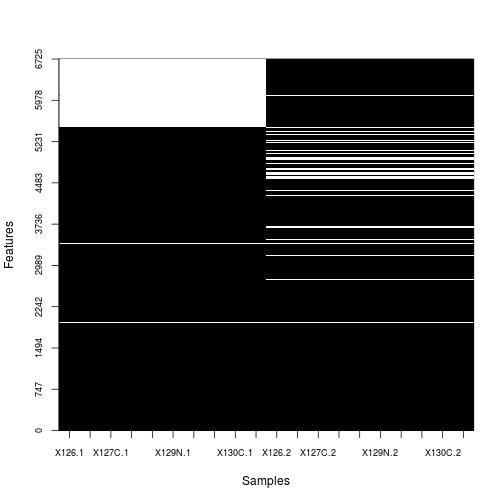
\includegraphics{figure/namap-1.png}
\caption{plot of chunk namap}
\end{figure}

We prefer to remove proteins that were not assayed in both of our two
replicated experiments. This is done with the \texttt{filterNA} function
that removes features that contain more than a certain proportion
(default is 0) missing values.

\begin{Shaded}
\begin{Highlighting}[]
\NormalTok{combined <-}\StringTok{ }\KeywordTok{filterNA}\NormalTok{(combined)}
\NormalTok{combined}
\end{Highlighting}
\end{Shaded}

\begin{verbatim}
## MSnSet (storageMode: lockedEnvironment)
## assayData: 5032 features, 20 samples 
##   element names: exprs 
## protocolData: none
## phenoData
##   sampleNames: X126.1 X127N.1 ... X131.2 (20 total)
##   varLabels: Replicate TMT.Reagent ... Iodixonal.Density (5 total)
##   varMetadata: labelDescription
## featureData
##   featureNames: Q9JHU4 Q9QXS1-3 ... Q9Z2R6 (5032 total)
##   fvarLabels: EntryName ProteinDescription ... ProteinCoverage2 (8
##     total)
##   fvarMetadata: labelDescription
## experimentData: use 'experimentData(object)'
## Annotation:  
## - - - Processing information - - -
## Combined [6725,20] and [6268,10] MSnSets Thu Sep 29 10:28:15 2016 
## Subset [6725,20][5032,20] Thu Sep 29 10:28:15 2016 
## Removed features with more than 0 NAs: Thu Sep 29 10:28:15 2016 
## Dropped featureData's levels Thu Sep 29 10:28:15 2016 
##  MSnbase version: 1.21.7
\end{verbatim}

When more than 2 data are to be combined and/or too many proteins were
not consistently assayed, leading to too many proteins being filtered
out, we suggest to implement an ensemble of classifiers voting on
protein-sub-cellular niche membership over the output of several
experiments (see section \emph{Supervised machine learning} for the
description of sub-cellular assignments).

\section{Quality Control}\label{quality-control}

Data quality is routinely examined through visualisation to verify that
sub-cellular niches have been separated along the gradient. Based on De
Duve's principle {[}@DeDuve:1981{]} proteins that co-localise exhibit
similar quantitation profiles across the gradient fractions employed.
One approach that has been widely used to visualise and inspect high
throughput mass spectrometry-based proteomics data is principal
components analysis (PCA). PCA is one of many dimensionality reduction
methods, that allow one to effectively summarise multi-dimensional data
in to 2 or 3 dimensions to enable visualisation. Very generally, the
original continuous multi-dimensional data is transformed into a set of
orthogonal components ordered according to the amount of variability
that they describe. The \texttt{plot2D} method in
\emph{\href{http://bioconductor.org/packages/pRoloc}{pRoloc}} allows one
to plot the principal components (PCs) of a dataset against one another,
by default the first two components are plotted on the x- and y-axis,
respectively (the \texttt{dims} argument can be used to plot other PCs).
If distinct clusters are observed, we assume that there is organellar
separation present in the data. Although, representing the
multi-dimensional data along a limited set of PCs does not give us a
hard quantitative measure of separation, it is extremely useful
summarising complex experimental information in one figure, to get an
simplified overview of the data.

In the code chunk below we produce a PCA plot of the mouse stem cell
dataset. One point on the plot represents one protein. We can indeed see
several distinct protein clusters. We specify \texttt{fcol = NULL},
which means not to consider any feature variable to annotate the
features (proteins) with colours. We will see later how to use this to
annotate the PCA plot with prior information about sub-cellular
localisation.

\begin{Shaded}
\begin{Highlighting}[]
\KeywordTok{library}\NormalTok{(}\StringTok{"pRoloc"}\NormalTok{)}
\KeywordTok{plot2D}\NormalTok{(hl, }\DataTypeTok{fcol =} \OtherTok{NULL}\NormalTok{, }\DataTypeTok{col =} \StringTok{"black"}\NormalTok{)}
\end{Highlighting}
\end{Shaded}

\begin{figure}[htbp]
\centering
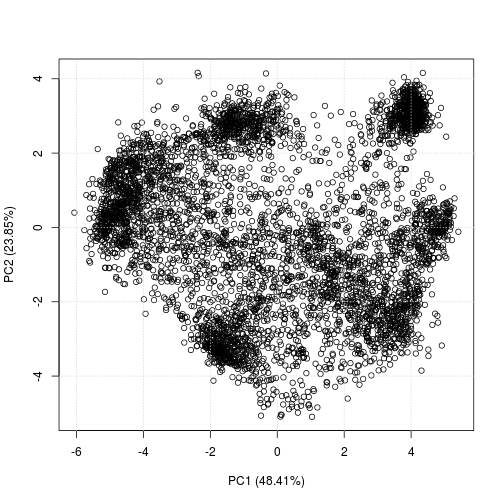
\includegraphics{figure/qcplot-1.png}
\caption{plot of chunk qcplot}
\end{figure}

In the first instance we advise one to visualise their data without any
annotation (i.e.~with \texttt{fcol = NULL}), before proceeding with data
annotation. The identification of well resolved clusters in the data,
constitutes an unbiased assessment of the data structure, demonstrating
the successful separation of sub-cellular clusters.

\textbf{TODO} There are other dimensionality reduction methods available
in the \texttt{plot2D} function, which can be parametrised with the
\texttt{method} argument. Advantages, disadvantages? See
\href{https://gist.github.com/mikelove/74bbf5c41010ae1dc94281cface90d32}{this}
very interesting gist with intriguing tSNE examples.

It is also useful to visualise the relative intensities along the
gradient to identify channels displaying particularly low yield. This
can be done using the \texttt{plotDist} and \texttt{boxplot} functions,
that plot the protein profiles occupancy along the gradient (we also
display the mean channel intensities) and a \texttt{boxplot} of the
column intensities. In the two plots displayed below, we re-order the
TMT channles to pair corresponding channels in the two replicates
(rather than ordering the channels by replicate).

\texttt{\{r qcbx, fig.width = 12\} par(mfrow = c(1, 2)) o \textless{}- order(hl\$Iodixonal.Density) plotDist(hl{[}, o{]}, pcol = "\#00000010") lines(colMeans(exprs(hl{[}, o{]})), col = "red", type = "b") boxplot(exprs(hl{[}, o{]}), las = 2)}

\section{Markers}\label{markers}

In the context of spatial proteomics, a marker protein is defined as a
well-known resident of a specific sub-cellular niche in a species
\emph{and} condition of interest. Applying this to machine learning
(ML), and specifically supervised learning, for the task of protein
localisation prediction, these markers constitute the labelled training
data to use as input to a classification analyses. Defining well-known
residents, and obtaining labelled training data for ML analyses can be
time consuming, but it is important to define markers that are
representative of the multivariate data space and on which a classifier
will be trained and generated.
\emph{\href{http://bioconductor.org/packages/pRoloc}{pRoloc}} provides a
convenience function, \texttt{addMarkers}, to directly add markers to a
\texttt{MSnSet} object, as demonstrated in the code chunk below. These
marker sets can be accessed using the \texttt{pRolocmarkers()} function.
Marker sets are stored as a simple named vector in R, and originate from
in-house user-defined sets of markers or from previous published studies
{[}@Gatto:2014b{]}, which are continuosly updated and integrated.

\begin{Shaded}
\begin{Highlighting}[]
\NormalTok{## List available marker sets}
\KeywordTok{pRolocmarkers}\NormalTok{()}
\end{Highlighting}
\end{Shaded}

\begin{verbatim}
## 7 marker lists available:
## Arabidopsis thaliana [atha]:
##  Ids: TAIR, 543 markers
## Drosophila melanogaster [dmel]:
##  Ids: Uniprot, 179 markers
## Gallus gallus [ggal]:
##  Ids: IPI, 102 markers
## Homo sapiens [hsap]:
##  Ids: Uniprot ID, 205 markers
## Mus musculus [mmus]:
##  Ids: Uniprot, 937 markers
## Saccharomyces cerevisiae [scer_sgd]:
##  Ids: SGD, 259 markers
## Saccharomyces cerevisiae [scer_uniprot]:
##  Ids: Uniprot Accession, 259 markers
\end{verbatim}

These markers can then be mapped to a \texttt{MSnSet}'s
\texttt{featureNames}. The mouse dataset used here has Uniprot IDs
stored as the \texttt{featureNames} (see
\texttt{head(featureNames(hl))}) and the names of the vector of the
mouse markers stored in
\emph{\href{http://bioconductor.org/packages/pRoloc}{pRoloc}}
(\texttt{mmus} markers) are also Uniprot IDs (see \texttt{head(mrk)} in
the code chunk below), so it is straightforward to match names between
the markers and the \texttt{MSnSet} instance using the
\texttt{addMarkers} function.

\begin{Shaded}
\begin{Highlighting}[]
\NormalTok{## Use mouse markers}
\NormalTok{mrk <-}\StringTok{ }\KeywordTok{pRolocmarkers}\NormalTok{(}\DataTypeTok{species =} \StringTok{"mmus"}\NormalTok{)}
\KeywordTok{head}\NormalTok{(mrk)}
\end{Highlighting}
\end{Shaded}

\begin{verbatim}
##                 P26039                 Q6PB66                 P11276 
##   "Actin cytoskeleton"        "Mitochondrion" "Extracellular matrix" 
##                 Q6PR54                 Q05793                 P19096 
##  "Nucleus - Chromatin" "Extracellular matrix"              "Cytosol"
\end{verbatim}

\begin{Shaded}
\begin{Highlighting}[]
\NormalTok{## Add mouse markers}
\NormalTok{hl <-}\StringTok{ }\KeywordTok{addMarkers}\NormalTok{(hl, mrk)}
\end{Highlighting}
\end{Shaded}

\begin{verbatim}
## Markers in data: 937 out of 5032
\end{verbatim}

\begin{verbatim}
## organelleMarkers
##            40S Ribosome            60S Ribosome      Actin cytoskeleton 
##                      27                      43                      13 
##                 Cytosol   Endoplasmic reticulum                Endosome 
##                      43                      95                      12 
##    Extracellular matrix         Golgi apparatus                Lysosome 
##                      10                      27                      33 
##           Mitochondrion     Nucleus - Chromatin Nucleus - Non-chromatin 
##                     383                      64                      85 
##              Peroxisome         Plasma membrane              Proteasome 
##                      17                      51                      34 
##                 unknown 
##                    4095
\end{verbatim}

If the naming between the marker sets and the \texttt{MSnSet} dataset
are different, one will have to convert and match the proteins according
to the appropriate identifier. Sometimes, we find the equivalent entry
name, Uniprot ID or accession number is stored with the data, which
makes conversion between identifers relatively straightforward. If this
is not the case however, conversion can be performed using
\emph{\href{http://bioconductor.org/packages/biomaRt}{biomaRt}}, the
Bioconductor
\href{http://bioconductor.org/help/workflows/annotation/Annotation_Resources/}{annotation
resouces} or any conversion softwares available online.

We now visualise these annotations along the PCA plot using the
\texttt{plot2D} function and then use the \texttt{addLegend} function to
map the marker classes to the pre-defined colours. We also display the
data along the first and seventh PCs using the \texttt{dims} argument.
Note that in this second call to the \texttt{plot2D} function, we have
omitted the \texttt{fcol} argument, as the \texttt{"markers"} feature
variable name is the default value. We choose to display PCs 1 and 7 to
illustrate that while upper principal components explain much less
variability in the data (2.23\% for PC7, as opposed to 48.41\% for PC1),
we see that the mitochondrial and peroxisome clusters can be
differenciated, despite the apparent overlap in the two first PCs.

\begin{Shaded}
\begin{Highlighting}[]
\KeywordTok{par}\NormalTok{(}\DataTypeTok{mfrow =} \KeywordTok{c}\NormalTok{(}\DecValTok{1}\NormalTok{, }\DecValTok{2}\NormalTok{))}
\KeywordTok{plot2D}\NormalTok{(hl, }\DataTypeTok{main =} \StringTok{"pRolocmarkers for mouse"}\NormalTok{)}
\KeywordTok{addLegend}\NormalTok{(hl, }\DataTypeTok{cex =} \NormalTok{.}\DecValTok{7}\NormalTok{)}
\KeywordTok{plot2D}\NormalTok{(hl, }\DataTypeTok{dims =} \KeywordTok{c}\NormalTok{(}\DecValTok{1}\NormalTok{, }\DecValTok{7}\NormalTok{), }\DataTypeTok{main =} \StringTok{"Marker resolution along PC 1 and 7"}\NormalTok{)}
\end{Highlighting}
\end{Shaded}

\begin{figure}[htbp]
\centering
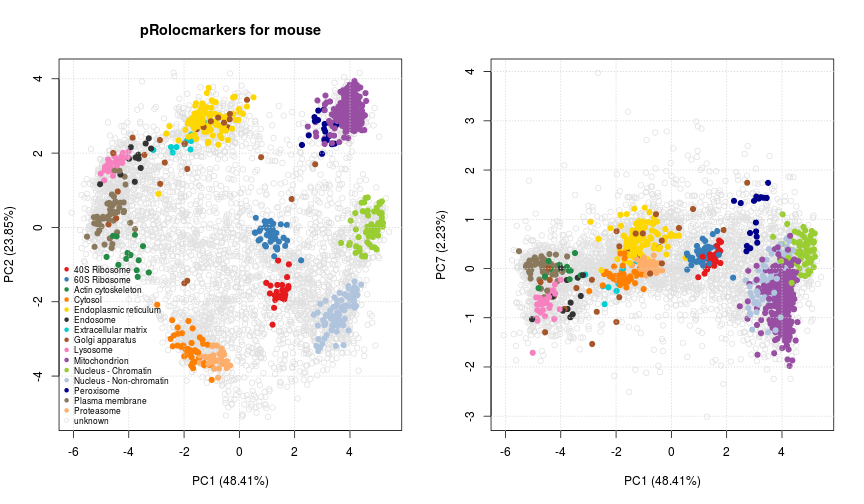
\includegraphics{figure/plotmarkers-1.png}
\caption{plot of chunk plotmarkers}
\end{figure}

The colours have been defined so as to enable to differenciate up to 30
classes. If more are provided, different character symbols (circles,
squares, \ldots{} and empty and solid symbols) are used. The colours and
the default plotting characters (solid dots for the markers and empty
circles for the features of unknown localisation) can of course be
changed, as described in the \texttt{setStockcol} manual page.

As demonstrated in {[}@hyper{]} and illustrated in the PCA plot above,
the Golgi apparatus proteins display a dynamic pattern, noting sets of
Golgi marker proteins that are distributed amongst other subcellular
structures, an observation supported by microscopy. As such, we are
going to reset the annotation of Golgi markers to unknown using the
\texttt{fDataTounknown} function. It is often used to replace empty
strings (``'') or missing values in the markers definition to a common
definition of \emph{unknown localisation}.

\begin{Shaded}
\begin{Highlighting}[]
\NormalTok{hl <-}\StringTok{ }\KeywordTok{fDataToUnknown}\NormalTok{(hl, }\DataTypeTok{from =} \StringTok{"Golgi apparatus"}\NormalTok{, }\DataTypeTok{to =} \StringTok{"unknown"}\NormalTok{)}
\KeywordTok{getMarkers}\NormalTok{(hl)}
\end{Highlighting}
\end{Shaded}

\begin{verbatim}
## organelleMarkers
##            40S Ribosome            60S Ribosome      Actin cytoskeleton 
##                      27                      43                      13 
##                 Cytosol   Endoplasmic reticulum                Endosome 
##                      43                      95                      12 
##    Extracellular matrix                Lysosome           Mitochondrion 
##                      10                      33                     383 
##     Nucleus - Chromatin Nucleus - Non-chromatin              Peroxisome 
##                      64                      85                      17 
##         Plasma membrane              Proteasome                 unknown 
##                      51                      34                    4122
\end{verbatim}

In general, the Gene Ontology (GO) {[}@Ashburner:2000{]}, and in
particular the cellular compartment (CC) namespace are a good starting
point for protein annotation and marker definition. It is important to
note however that automatic retrieval of sub-cellular localisation
information, from
\emph{\href{http://bioconductor.org/packages/pRoloc}{pRoloc}} or
elsewhere, is only the beginning in defining a marker set for downstream
analyses. Expert curation is vital to check that any annotation added is
in the correct context for the the biological question under
investigation.

Another useful visualisation that relies on marker annotation is the
representation of the protein profiles occupancy along the gradient
using the \texttt{plotDist} function. While the PCA plot enables to
efficiently visualise the complete dataset and assess the relative
separation of different sub-cellular niches, comparing profiles of a few
marker clusters is useful to assess how exactly they differ (in terms of
peak channels, for example). Below, we plot the profile of the
mitochondrial and peroxisome markers to highlight the differences in
profiles between these two sets of markers along the 6th and 7th
channels, as represented above along the 7th PC on the PCA plot.

\begin{Shaded}
\begin{Highlighting}[]
\NormalTok{hlo <-}\StringTok{ }\NormalTok{hl[, }\KeywordTok{order}\NormalTok{(hl$Iodixonal.Density)]}
\KeywordTok{plotDist}\NormalTok{(hlo[}\KeywordTok{fData}\NormalTok{(hlo)$markers ==}\StringTok{ "Mitochondrion"}\NormalTok{, ],}
         \DataTypeTok{pcol =} \StringTok{"purple"}\NormalTok{, }\DataTypeTok{fractions =} \StringTok{"Fraction.No"}\NormalTok{)}
\KeywordTok{title}\NormalTok{(}\DataTypeTok{main =} \StringTok{"Marker occupancy profiles along the gradient"}\NormalTok{)}
\KeywordTok{matlines}\NormalTok{(}\KeywordTok{t}\NormalTok{(}\KeywordTok{exprs}\NormalTok{(hlo[}\KeywordTok{fData}\NormalTok{(hlo)$markers ==}\StringTok{ "Peroxisome"}\NormalTok{, ])),}
         \DataTypeTok{lty =} \DecValTok{1}\NormalTok{, }\DataTypeTok{col =} \StringTok{"darkblue"}\NormalTok{, }\DataTypeTok{type =} \StringTok{"l"}\NormalTok{)}
\KeywordTok{legend}\NormalTok{(}\StringTok{"topleft"}\NormalTok{, }\KeywordTok{c}\NormalTok{(}\StringTok{"Mitochondrion"}\NormalTok{, }\StringTok{"Peroxisome"}\NormalTok{),}
       \DataTypeTok{lty =} \DecValTok{1}\NormalTok{, }\DataTypeTok{col =} \KeywordTok{c}\NormalTok{(}\StringTok{"purple"}\NormalTok{, }\StringTok{"blue"}\NormalTok{), }\DataTypeTok{bty =} \StringTok{"n"}\NormalTok{)}
\end{Highlighting}
\end{Shaded}

\begin{figure}[htbp]
\centering
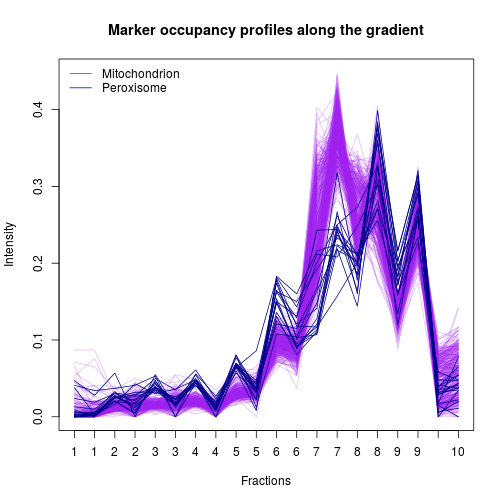
\includegraphics{figure/plotDist-1.png}
\caption{plot of chunk plotDist}
\end{figure}

\textbf{TODO} Possibly mention \texttt{plot3D} and \texttt{mrkHClust},
although these are only available in the development version.

\section{Replication}\label{replication}

With the aim of maximising the sub-cellular resolution and,
consequently, the reliability in protein sub-cellular assignments, we
follow the advice in {[}@Trotter:2010{]} and combine replicated spatial
proteomics experiments as described above. Indeed, Trotter et al. have
shown a significant improvement in protein--organelle association upon
direct combination of single experiments, in particular when these
resolve different subcellular niches.

Direct comparisons of individual channels in replicated experiments does
not provide an adequate, goal-driven assessment of different
experiments. Indeed, due to the nature of the experiment and gradient
fraction collection, the quantitative channels do not correspond to
identical selected fractions along the gradient. As can be seen in the
table below (taken from the \texttt{hyperLOPIT}'s \texttt{pData},
focusing on channels 7 to 10), different sets of gradient fractions are
pooled to obtain enough material and optimise acurate quantitation.

The more relevant comparison unit is not a single channel, but rather
the complete protein occupancy profiles, which are best visualised as
experiment-wide on a PCA plot. As such, we prefer to focus on the
direct, qualitative comparison of individual replicate PCA plots,
assuring that each displays acceptable sub-cellular resolution. Note
that in the code chunk below, we mirror the x-axis to represent the two
figures with the same orientation.

\begin{Shaded}
\begin{Highlighting}[]
\KeywordTok{par}\NormalTok{(}\DataTypeTok{mfrow =} \KeywordTok{c}\NormalTok{(}\DecValTok{1}\NormalTok{, }\DecValTok{2}\NormalTok{)) }
\KeywordTok{plot2D}\NormalTok{(hl[, hl$Replicate ==}\StringTok{ }\DecValTok{1}\NormalTok{], }\DataTypeTok{main =} \StringTok{"Replicate 1"}\NormalTok{) }
\KeywordTok{plot2D}\NormalTok{(hl[, hl$Replicate ==}\StringTok{ }\DecValTok{2}\NormalTok{], }\DataTypeTok{main =} \StringTok{"Replicate 2"}\NormalTok{, }\DataTypeTok{mirrorX =} \OtherTok{TRUE}\NormalTok{) }
\end{Highlighting}
\end{Shaded}

\begin{figure}[htbp]
\centering
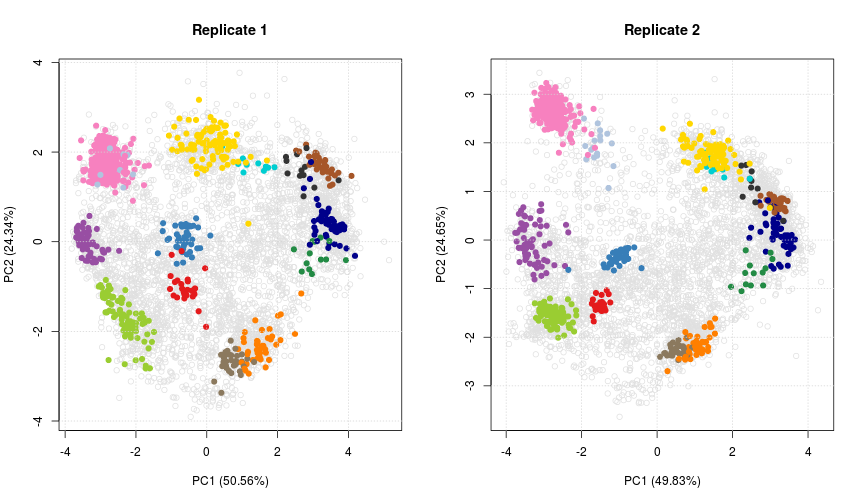
\includegraphics{figure/plot2Drep-1.png}
\caption{plot of chunk plot2Drep}
\end{figure}

\section{Interactive visualisation}\label{interactive-visualisation}

Visualisation and data exploration is an important aspect of data
analyses allowing one to shed light on data structure and patterns of
interest. Using the
\emph{\href{http://bioconductor.org/packages/pRolocGUI}{pRolocGUI}}
package we can interactively visualise, explore and interrogate
quantitative spatial proteomics data. The
\emph{\href{http://bioconductor.org/packages/pRolocGUI}{pRolocGUI}}
package is currently under active development and it relies on the
\texttt{shiny} framework for reactivity and interactivity. The package
currently distributes 3 different GUI's (``main'' (default), ``compare''
or ``compare'') which are wrapped and launched by the \texttt{pRolocVis}
function. In the below code chunk we lauch the main app (note, we do not
need to specify the argument, \texttt{app = "main"} as it is the
default).

\begin{Shaded}
\begin{Highlighting}[]
\KeywordTok{library}\NormalTok{(}\StringTok{"pRolocGUI"}\NormalTok{)}
\KeywordTok{pRolocVis}\NormalTok{(hl)}
\end{Highlighting}
\end{Shaded}

\begin{figure}[htbp]
\centering
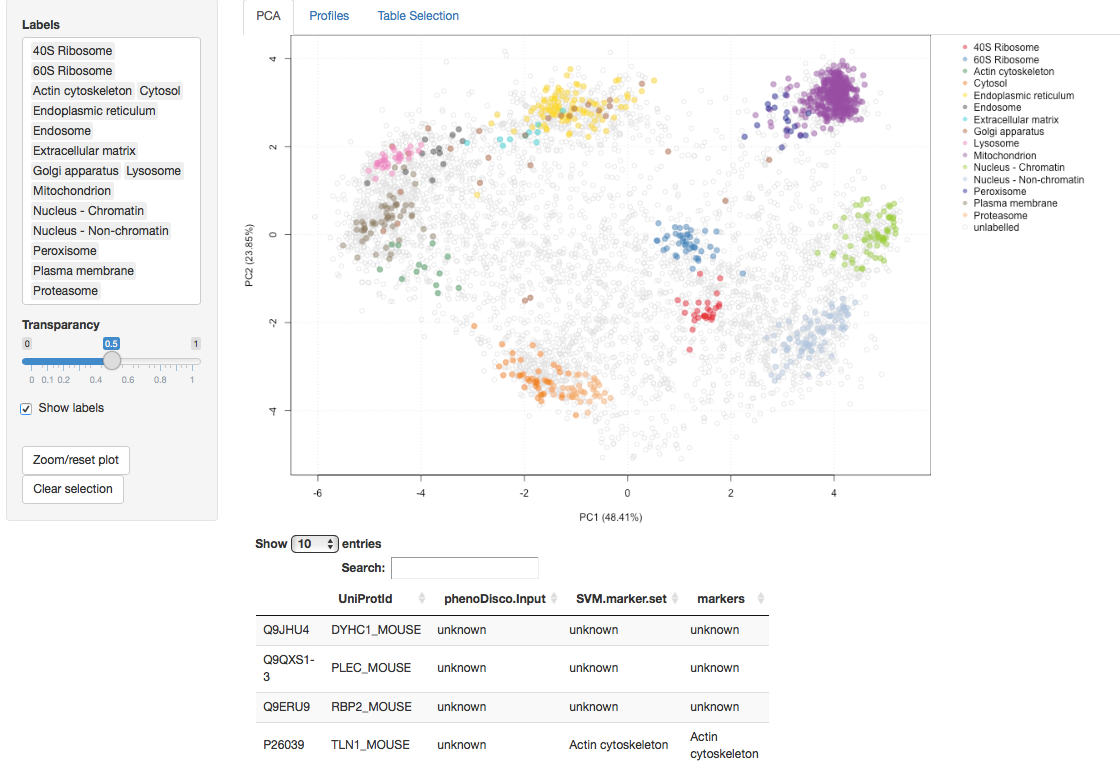
\includegraphics{./Figures/mainapp.png}
\caption{A screen shot of clickable interface and zoomable PCA plot of
the main app in the
\emph{\href{http://bioconductor.org/packages/pRolocGUI}{pRolocGUI}}
package.}
\end{figure}

As diplayed in the screenshot above, the ``main'' application is
designed for exploratory data analysis and is divied into 3 tabs: (1)
PCA, (2) Profiles and (3) Table selection. The default view upon loading
is the PCA tab, which features a clickable interface and zoomable PCA
plot with an interactive data table for displaying the quantitation
information. Particular proteins of interest can be highlighted using
the text search box. There is also an alternate profiles tab for
visualisation of the protein profiles, which can be used to examine the
patterns of proteins of interest. The Table selection tab provides an
interface to control data table column selection.

The ``compare'' application is useful for examining two replicate
experiments, or two experiments from different conditions, treatments
etc. The compare application is called by default if the input object to
\texttt{pRolocVis} is a \texttt{MSnSetList} of 2 \texttt{MSnSets}, but
it can also be specified by calling the argument
\texttt{app = "compare"}. For example, in the code chunk below we first
create a \texttt{MSnSetList} of replicates 1 and 2 of the hyperLOPIT
data, this is then passed to \texttt{pRolocVis}.

\begin{Shaded}
\begin{Highlighting}[]
\KeywordTok{data}\NormalTok{(hyperLOPIT2015ms3r1)}
\KeywordTok{data}\NormalTok{(hyperLOPIT2015ms3r2)}
\NormalTok{mydata <-}\StringTok{ }\KeywordTok{MSnSetList}\NormalTok{(}\KeywordTok{list}\NormalTok{(hyperLOPIT2015ms3r1, hyperLOPIT2015ms3r2))}
\KeywordTok{pRolocVis}\NormalTok{(mydata, }\DataTypeTok{app =} \StringTok{"compare"}\NormalTok{)}
\end{Highlighting}
\end{Shaded}

\begin{figure}[htbp]
\centering
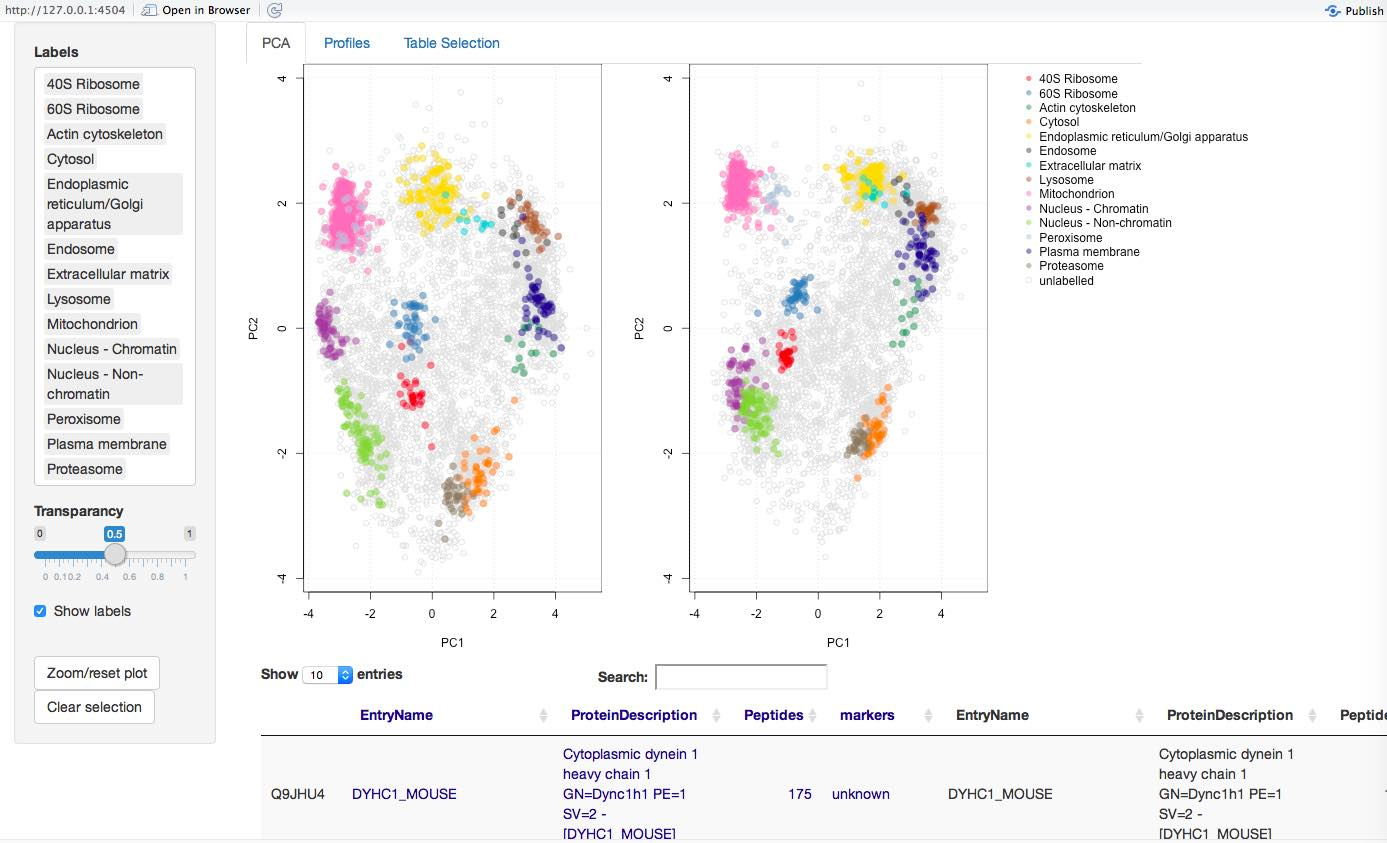
\includegraphics{./Figures/SS_Compare1.jpg}
\caption{The compare application, main panel}
\end{figure}

The comparison app loads the two PCA plots side-by-side. Only common
proteins between the two data sets are displayed. As per the main
application proteins can be searched, identified and highlighted on both
PCA plots and in the dedicated profiles tab. One key feature of the
compare application is the ability to re-map the second dataset onto the
PCA data space of the first (reference) data set (see
\texttt{?pRolocVis} and the argument \texttt{remap = TRUE}). Using the
first dataset as the reference set, PCA is carried out on the first
dataset and the standard deviations of the principal components
(i.e.~the square roots of the eigenvalues of the covariance/correlation
matrix) and the matrix of variable loadings (i.e.~a matrix whose columns
contain the eigenvectors) are stored and then used to calculate the
principal components of the second dataset. Both datasets are scaled and
centered in the usual way. The first dataset appears on the left, and
the second re-mapped data appears on the right. The order of the first
(the reference data for remapping) and second dataset can be changed
through regeneration/re-ordering of the \texttt{MSnSetList} object.

The final application ``classify'', has been designed to view machine
learning classification results according to user-specified thresholds
for the assignment of proteins to its sub-cellular location, this is
discussed later in the subsection \hyperref[thresholding]{thresholding}
in the \hyperref[supervised-machine-learning]{supervised machine
learning section}.

\section{Novelty Detection}\label{novelty-detection}

The extraction of sub-cellular protein clusters can be difficult owing
to the limited number of marker proteins that exist in databases and
elsewhere. Furthermore, given the vast complexity of the cell, automatic
annotation retrieval does not always give a full representation of the
true sub-cellular diversity in the data. For downstream analyses, such
as supervised machine learning, it is desirable to obtain reliable
markers that cover as many sub-cellular niches as possible, as these
markers are directly used in the training phase of the ML
classification. We find that a lack of sub-cellular diversity in the
labelled training data leads to prediction errors, as unlabelled
instances can only be assigned to a class that exists in the training
data {[}@Breckels:2013{]}. In such scenarios novelty detection can be
useful to identify data-specific sub-cellular groupings such as
organelles and protein complexes. The phenotype discovery (phenoDisco)
algorithm {[}@Breckels:2013{]} is one such method and is available in
\emph{\href{http://bioconductor.org/packages/pRoloc}{pRoloc}}. It is an
iterative semi-supervised learning method that combines the
classification of proteins on existing labelled data with the detection
of new clusters.

In addition to extracting new phenotypes, novelty detection methods are
also useful for confirming the presence of known or postulated clusters
in an unbiased fashion. For example, in {[}@hyper{]} the
\texttt{phenoDisco} algorithm was used to confirm the data-specific
presence of the nucleus and nucleus sub-compartments. In the code chunk
below, we demonstrate how to do this analysis, highlighting some of the
optional arguments and parameters available for phenotype extraction and
give some advice on how to interpret the output.

As the \texttt{phenoDisco} algorithm is semi-supervised it uses both
labelled (markers) and unlabelled data to explore the data structure and
find new sub-cellular data clusters. Thus the first step is to define
some input labelled data i.e.~markers, that the algorithm will use as
input for the supervised learning aspect of the algorithm. As described
in {[}@hyper{]} we define a set of markers to use as input for the
analyses that cover well-known residents from three distinct organelle
structures; the mitochondria, plasma membrane and ER, and from three
well-known and abundant protein complexes; the proteasome and two
ribosomal subunits, 40S and 60S. These input markers are stored in the
\texttt{featureData} column of \texttt{hl} where
\texttt{fcol = "phenoDisco.Input"}. We can use the convenience accessor
function \texttt{getMarkers} to print out a table of the markers
contained in this marker set. These initial markers were manually
curated using information from the UniProt database, the Gene Ontology
and the literature.

\begin{Shaded}
\begin{Highlighting}[]
\KeywordTok{getMarkers}\NormalTok{(hl, }\DataTypeTok{fcol =} \StringTok{"phenoDisco.Input"}\NormalTok{)}
\end{Highlighting}
\end{Shaded}

\begin{verbatim}
## organelleMarkers
##                          40S Ribosome 
##                                    26 
##                          60S Ribosome 
##                                    43 
## Endoplasmic reticulum/Golgi apparatus 
##                                    76 
##                         Mitochondrion 
##                                   261 
##                       Plasma membrane 
##                                    50 
##                            Proteasome 
##                                    34 
##                               unknown 
##                                  4542
\end{verbatim}

In the code chunk below we show how to run the \texttt{phenoDisco}
function and return a novelty detection result, according to the
specified parameters. The algorithm parameters \texttt{times},
\texttt{GS} and \texttt{p} are passed to the function, along with the
\texttt{fcol} to tell the algorithm where the input training data is
contained.

\begin{Shaded}
\begin{Highlighting}[]
\NormalTok{## As per Christoforou et al (2016), }
\NormalTok{hl <-}\StringTok{ }\KeywordTok{phenoDisco}\NormalTok{(hl, }\DataTypeTok{fcol =} \StringTok{"phenoDisco.Input"}\NormalTok{, }
                 \DataTypeTok{times =} \DecValTok{200}\NormalTok{, }
                 \DataTypeTok{GS =} \DecValTok{60}\NormalTok{)}
\end{Highlighting}
\end{Shaded}

\emph{Note: We do not evaluate this code chunk in this document as the
algorithm is computational intensive and best parallelised over multiple
workers. This phenoDisco analysis took \textasciitilde{}24 hours to
complete when parallelised over 40 workers.}

The argument \texttt{times} indicated the number of times we run
unsupervied Gaussian Mixture Modelling before defining a new phenotype
cluster. The recommended minimum and default value is 100. In the above
code chunk we increase the value to \texttt{times = 200} as we have
found for larger datasets (e.g.~5000+ proteins) a higher times is
requried for convergence. \texttt{GS} defines the minimum number of
proteins allowed per new data cluster and thus heavily influences what
type of new clusters are extracted. For example, if a user is interesed
in the detection of small complexes they may wish to use a small
\texttt{GS = 10}, or \texttt{= 20} etc. If they wish to detect larger
more abundant sub-cellular niches a much higher \texttt{GS} would be
preferable. Specifying a small \texttt{GS} can be more time consuming
than using a larger \texttt{GS}, and there is a trade off between
finding interesting small complexes and those that may not be of
interest as we find there is a tendancy to find more noise when using a
small \texttt{GS} compared to using a higher one.

One may also consider increasing the search space for new data clusters
by increasing the value of the parameter \texttt{G}. This defines the
number of GMM components to test and fit; the default is
\texttt{G = 1:9} (\texttt{mclust}'s default). One should note that the
decreasing the \texttt{GS}, and increasing the values of the arguments
\texttt{times}, \texttt{G} (among other function arguments, see
\texttt{?phenoDisco}) will heavily influence (increase) the total time
taken to run the algorithm. \texttt{phenoDisco} supports parallelisation
and we strongly suggest you make use of a parallel processing to run
these analyses (different backends can be set with argument
\texttt{BPPARAM}).

The ouput of running the \texttt{phenoDisco} algorithm is a
\texttt{MSnSet} containing the new data clusters, appended to the
\texttt{featureData} under the name \texttt{pd}. We can see by typing
\texttt{hl@processingData} directly into the console the processing
information has been updated to the \texttt{MSnSet} recording the
parameters that were used to run the analyses. This is handy for keeping
track of data analyses. The results can be displayed by using the
\texttt{getMarkers} function. We see that 5 new phenotype data clusters
were found.

\begin{Shaded}
\begin{Highlighting}[]
\NormalTok{hl}
\end{Highlighting}
\end{Shaded}

\begin{verbatim}
## MSnSet (storageMode: lockedEnvironment)
## assayData: 5032 features, 20 samples 
##   element names: exprs 
## protocolData: none
## phenoData
##   sampleNames: X126 X127N ... X131.1 (20 total)
##   varLabels: Replicate Tag Gradient.Fraction Iodixonal.Density
##   varMetadata: labelDescription
## featureData
##   featureNames: Q9JHU4 Q9QXS1-3 ... Q9Z2R6 (5032 total)
##   fvarLabels: uniprot.accession uniprot.id ... pd (27 total)
##   fvarMetadata: labelDescription
## experimentData: use 'experimentData(object)'
## Annotation:  
## - - - Processing information - - -
## Added markers from  'mrk' marker vector. Thu Sep 29 10:28:15 2016 
## Added markers from  'pdres' marker vector. Thu Sep 29 10:28:17 2016 
##  MSnbase version: 1.99.2
\end{verbatim}

\begin{Shaded}
\begin{Highlighting}[]
\KeywordTok{getMarkers}\NormalTok{(hl, }\DataTypeTok{fcol =} \StringTok{"pd"}\NormalTok{)}
\end{Highlighting}
\end{Shaded}

\begin{verbatim}
## organelleMarkers
##                          40S Ribosome 
##                                   106 
##                          60S Ribosome 
##                                    95 
## Endoplasmic reticulum/Golgi apparatus 
##                                   393 
##                         Mitochondrion 
##                                   525 
##                           Phenotype 1 
##                                   300 
##                           Phenotype 2 
##                                   253 
##                           Phenotype 3 
##                                   203 
##                           Phenotype 4 
##                                    74 
##                           Phenotype 5 
##                                    91 
##                       Plasma membrane 
##                                   421 
##                            Proteasome 
##                                    92 
##                               unknown 
##                                  2479
\end{verbatim}

We can plot the results using the \texttt{plot2D} function.

\begin{Shaded}
\begin{Highlighting}[]
\NormalTok{## Re-order the colours for the phenoDisco output}
\NormalTok{cl <-}\StringTok{ }\KeywordTok{getMarkerClasses}\NormalTok{(hl, }\StringTok{"pd"}\NormalTok{)}
\NormalTok{cols <-}\StringTok{ }\KeywordTok{getStockcol}\NormalTok{()[}\KeywordTok{seq}\NormalTok{(cl)]}
\NormalTok{ind <-}\StringTok{ }\KeywordTok{grep}\NormalTok{(}\StringTok{"Pheno"}\NormalTok{, cl, }\DataTypeTok{invert =} \OtherTok{TRUE}\NormalTok{)}
\NormalTok{cols[ind] <-}\StringTok{ }\KeywordTok{getStockcol}\NormalTok{()[}\KeywordTok{seq}\NormalTok{(cl)][}\DecValTok{1}\NormalTok{:}\KeywordTok{length}\NormalTok{(ind)]}
\NormalTok{cols[-ind] <-}\StringTok{ }\KeywordTok{getStockcol}\NormalTok{()[}\KeywordTok{seq}\NormalTok{(cl)][(}\KeywordTok{length}\NormalTok{(ind) +}\StringTok{ }\DecValTok{1}\NormalTok{):}\KeywordTok{length}\NormalTok{(cl)]}

\NormalTok{## Plot the input and output}
\KeywordTok{par}\NormalTok{(}\DataTypeTok{mfrow =} \KeywordTok{c}\NormalTok{(}\DecValTok{1}\NormalTok{, }\DecValTok{2}\NormalTok{))}
\KeywordTok{plot2D}\NormalTok{(hl, }\DataTypeTok{fcol =} \StringTok{"phenoDisco.Input"}\NormalTok{, }
       \DataTypeTok{main =} \StringTok{"phenoDisco input markers"}\NormalTok{, }\DataTypeTok{col =} \KeywordTok{getStockcol}\NormalTok{()[}\DecValTok{1}\NormalTok{:}\DecValTok{6}\NormalTok{])}
\KeywordTok{addLegend}\NormalTok{(hl, }\DataTypeTok{fcol =} \StringTok{"phenoDisco.Input"}\NormalTok{, }\DataTypeTok{cex =} \NormalTok{.}\DecValTok{7}\NormalTok{)}
\KeywordTok{plot2D}\NormalTok{(hl, }\DataTypeTok{fcol =} \StringTok{"pd"}\NormalTok{, }\DataTypeTok{main =} \StringTok{"phenoDisco output"}\NormalTok{, }\DataTypeTok{col =} \NormalTok{cols)}
\KeywordTok{addLegend}\NormalTok{(hl, }\DataTypeTok{fcol =} \StringTok{"pd"}\NormalTok{, }\DataTypeTok{cex =} \NormalTok{.}\DecValTok{7}\NormalTok{, }\DataTypeTok{col =} \NormalTok{cols)}
\end{Highlighting}
\end{Shaded}

\begin{figure}[htbp]
\centering
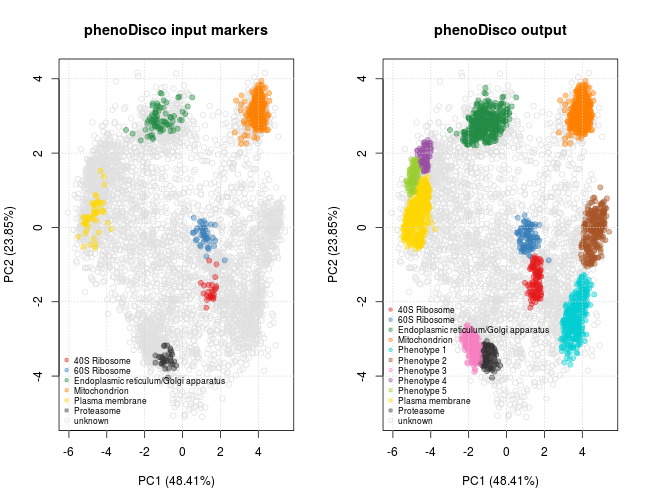
\includegraphics{figure/plotPDres-1.png}
\caption{plot of chunk plotPDres}
\end{figure}

The five new phenotype data clusters can be extracted and examined. In
the code chunk below we write the results to a .csv file. We use the
argument \texttt{fDataCols} to specify which columns of the
\texttt{featureData} to write.

\begin{Shaded}
\begin{Highlighting}[]
\KeywordTok{fData}\NormalTok{(hl)$pd <-}\StringTok{ }\KeywordTok{as.character}\NormalTok{(}\KeywordTok{fData}\NormalTok{(hl)$pd)}
\KeywordTok{write.exprs}\NormalTok{(hl, }\DataTypeTok{fDataCols =} \StringTok{"pd"}\NormalTok{, }\DataTypeTok{file =} \StringTok{"pd-results.csv"}\NormalTok{, }\DataTypeTok{sep =} \StringTok{","}\NormalTok{)}
\end{Highlighting}
\end{Shaded}

We can also examine the each phenotype intercatively and visualise their
protein profiles by using the \texttt{pRolocVis} function in the
\texttt{pRolocGUI}. We found that phenotype 1 was enriched in nucleus
associated proteins, phenotype 2 in chromatin associated proteins,
phenotype 3 in cytosolic and phenotypes 4 and 5 in lysosomal and
endosomal proteins.

\begin{Shaded}
\begin{Highlighting}[]
\KeywordTok{pRolocVis}\NormalTok{(hl, }\DataTypeTok{fcol =} \StringTok{"pd"}\NormalTok{)}
\end{Highlighting}
\end{Shaded}

\hyperdef{}{supervised-machine-learning}{\section{Supervised machine
learning}\label{supervised-machine-learning}}

Supervised machine learning, also known as classification, is an
essential tool for the assignment of proteins to distinct sub-cellular
niches. Using a set of labelled training examples i.e.~markers, we can
train a machine learning classifier to learn a mapping between the data
i.e.~the quantitative protein profiles, and a known localisation. The
trained classifier can then be used to predict the localisation of a
protein of unknown localisation, based on its observed protein profile.
To date, this method has been extensively used in spatial quantitative
proteomics to assign thousands of proteins to distinct sub-cellular
niches {[}@hyper; @Groen:2014; @Trotter:2010; @Hall:2009; @Dunkley:2006;
@Tan:2009{]}.

There are several classification algorithms readily available in
\texttt{pRoloc}, which are documented in the dedicated
\href{http://bioconductor.org/packages/release/bioc/vignettes/pRoloc/inst/doc/pRoloc-ml.pdf}{\texttt{pRoloc}
machine learning techniques vignette}. We find the general tendancy to
be that it is not the choice of classifier, but the improper
optimisation of the algorithmic parameters, that limits classification
accuracy. Before employing any classification algorithm and generating a
model on the training data, one must first find the optimal parameters
for the algorithm of choice.

\subsection{Optimisation}\label{optimisation}

In the code chunk below we employ the use of a Support Vector Machine
(SVM) to learn a classifier on the labelled training data. As previously
mentioned one first needs to train the classifiers parameters before an
algorithm can be used to predict the class labels of the proteins with
unknown location. One of the most common ways to optimise the parameters
of a classifier is to partition the labelled data in to training and
testing subsets. In this framework parameters are tested via a grid
search using cross-validation on the training partition. The best
parameters chosen from the cross-validation stage are then used to build
a classifier to predict the class labels of the protein profiles on the
test partition. Observed and expected classication results can be
compared, and then used to assess how well a given model works by
getting an estimate of the classiers ability to achieve a good
generalisation i.e.~that is given an unknown example predict its class
label with high accuracy. In \texttt{pRoloc} algorithmic performance is
estimated using stratified 80/20 partitioning for the training/testing
subsets respectively, in conjuction with five-fold cross-validation in
order to optimise the free parameters via a grid search. This procedure
is usually repeated 100 times and then the best parameter(s) are
selected upon investigation of classifier accuracy, here we use the
harmonic mean of precision and recall; the macro F1 score. In the code
chunk below we demonstrate how to optimise the free parameters;
\texttt{sigma} and \texttt{cost}, of a classical SVM classifier with a
Gaussian kernel using the function \texttt{svmOptimisation}. As the
number of labelled instances per class varies from organelle to
organelle, we can account for class imbalance by setting specific class
weights when generating the SVM model. Below the weights, \texttt{w} are
set to be inversely proportional to the class frequencies.

\begin{Shaded}
\begin{Highlighting}[]
\NormalTok{w <-}\StringTok{ }\KeywordTok{table}\NormalTok{(}\KeywordTok{getMarkers}\NormalTok{(hl, }\DataTypeTok{verbose =} \OtherTok{TRUE}\NormalTok{))}
\end{Highlighting}
\end{Shaded}

\begin{verbatim}
## organelleMarkers
##            40S Ribosome            60S Ribosome      Actin cytoskeleton 
##                      27                      43                      13 
##                 Cytosol   Endoplasmic reticulum                Endosome 
##                      43                      95                      12 
##    Extracellular matrix                Lysosome           Mitochondrion 
##                      10                      33                     383 
##     Nucleus - Chromatin Nucleus - Non-chromatin              Peroxisome 
##                      64                      85                      17 
##         Plasma membrane              Proteasome                 unknown 
##                      51                      34                    4122
\end{verbatim}

\begin{Shaded}
\begin{Highlighting}[]
\NormalTok{w <-}\StringTok{ }\DecValTok{1}\NormalTok{/w[}\KeywordTok{names}\NormalTok{(w) !=}\StringTok{ "unknown"}\NormalTok{]}
\end{Highlighting}
\end{Shaded}

\begin{Shaded}
\begin{Highlighting}[]
\NormalTok{## 100 rounds of optimisation with five-fold cross-validation}
\NormalTok{params <-}\StringTok{ }\KeywordTok{svmOptimisation}\NormalTok{(hl, }\DataTypeTok{fcol =} \StringTok{"markers"}\NormalTok{,}
                          \DataTypeTok{times =} \DecValTok{100}\NormalTok{, }\DataTypeTok{xval =} \DecValTok{5}\NormalTok{,}
                          \DataTypeTok{class.weights =} \NormalTok{w)}
\end{Highlighting}
\end{Shaded}

As mentioned previously, we reply on the default feature variable
\texttt{"markers"} to define the class labels and hence can ommit it. To
use another feature variables, one need to explicitly specify its name
using the \texttt{fcol} argument (for example
\texttt{fcol = "markers2"}).

The output \texttt{params} is an object of class \texttt{GenRegRes}; a
dedicated container for the storage of the design and results from a
machine learning optimisation. To assess classifier performance we can
examine the macro F1 scores and the most frequently chosen parameters. A
high macro F1 score indicates that the marker proteins in the test
dataset are consistently and correctly assigned by the the algorithm.
Often more than one parameter or set of parameters gives rise to the
best generalisation accuracy. As such it is always important to
investigate the model parameters and critically assess the best choice.
The best choice may not be as simple as the parameter set that gives
rise to the highest macro F1 score and one must be careful to avoid
overfitting and to choose parameters wisely.

\begin{Shaded}
\begin{Highlighting}[]
\NormalTok{(best <-}\StringTok{ }\KeywordTok{getParams}\NormalTok{(params))}
\KeywordTok{plot}\NormalTok{(params)}
\KeywordTok{levelPlot}\NormalTok{(params)}
\end{Highlighting}
\end{Shaded}

\begin{figure}[htbp]
\centering
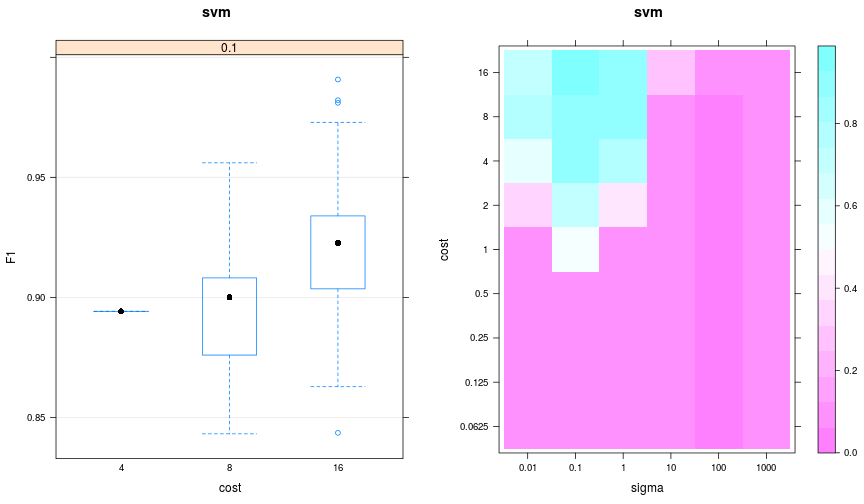
\includegraphics{figure/visualiseOptHide-1.png}
\caption{plot of chunk visualiseOptHide}
\end{figure}

By using the function \texttt{getParams} we can extract the best set of
parameters. Currently, \texttt{getParams} retrieves the first best set
is automatically but users are encouraged to critically assess whether
this is the most wise choice by visualising the results using the
methods \texttt{plot} and \texttt{levelPlot}. The \texttt{plot} method
for \texttt{GenRegRes} object shows the respective distributions of the
100 macro F1 scores for the best cost/sigma parameter pairs, and
\texttt{levelPlot} shows the averaged macro F1 scores, for the full
range of parameter values. Once we have selected the best parameters we
can then use them to build a classifier from the labelled marker
proteins.

\subsection{Classification}\label{classification}

We can use the function \texttt{svmClassification} to return a
classification result for all unlabelled instances in the dataset
corresponding to their most likely sub-cellular location. The algorithm
parameters are passed to the function, along with the class weights. As
above, \texttt{fcol} can be ignored as we use the labels defined in the
default \texttt{"markers"} feature variable.

\begin{Shaded}
\begin{Highlighting}[]
\NormalTok{hl <-}\StringTok{ }\KeywordTok{svmClassification}\NormalTok{(hl, params,}
                        \DataTypeTok{class.weights =} \NormalTok{w,}
                        \DataTypeTok{fcol =} \StringTok{"markers"}\NormalTok{)}
\end{Highlighting}
\end{Shaded}

Automatically, the output of the above classification; the organelle
predictions and assignment scores, are stored in the
\texttt{featureData} slot of the \texttt{MSnSet}. In this case, they are
given the labels \texttt{svm} and \texttt{svm.scores} for the
predictions and scores respectively. The resultant predictions can be
visualised using \texttt{plot2D}. In the code chunk below
\texttt{plot2D} is called to generate a PCA plot of the data and
\texttt{fcol} is used to specify where the new assignments are located
e.g. \texttt{fcol =  "svm"}.

Additionally, when calling \texttt{plot2D} we can use the \texttt{cex}
argument to change the size of each point on the plot (where one point
represents one protein) to be inversely proportional to the SVM score.
This gives an initial overview of the high scoring localisations from
the SVM predictions.

\begin{Shaded}
\begin{Highlighting}[]
\NormalTok{## set point size of each protein to be inversely proportional to the}
\NormalTok{ptsze <-}\StringTok{ }\KeywordTok{exp}\NormalTok{(}\KeywordTok{fData}\NormalTok{(hl)$svm.scores) -}\StringTok{ }\DecValTok{1}

\NormalTok{## plot new predictions}
\KeywordTok{plot2D}\NormalTok{(hl, }\DataTypeTok{fcol =} \StringTok{"svm"}\NormalTok{, }\DataTypeTok{cex =} \NormalTok{ptsze)}
\KeywordTok{addLegend}\NormalTok{(hl, }\DataTypeTok{fcol =} \StringTok{"svm"}\NormalTok{, }\DataTypeTok{where =} \StringTok{"bottomleft"}\NormalTok{, }\DataTypeTok{bty =} \StringTok{"n"}\NormalTok{, }\DataTypeTok{cex =} \NormalTok{.}\DecValTok{5}\NormalTok{)}
\end{Highlighting}
\end{Shaded}

\begin{figure}[htbp]
\centering
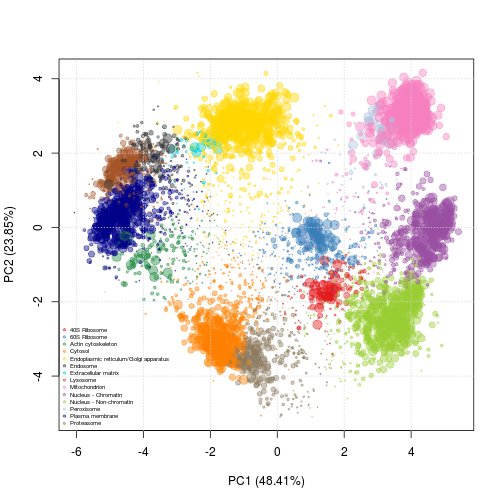
\includegraphics{figure/plotSVM-1.png}
\caption{plot of chunk plotSVM}
\end{figure}

The adjustment of the point size intuitively confers important
information that is more difficult to defined formally, but that we will
address in the next section. The classifier (SVM in our case, but this
is also valid of other classifiers) defines boundaries based on the
labelled marker proteins. These class/organelle boundaries define how
non-assigned proteins are classified and with what confidence.
\textbf{TODO} explain how choosing markers positively/negatively affects
this, and relation with thresholding.

\hyperdef{}{thresholding}{\subsection{Thresholding}\label{thresholding}}

It is common when applying a supervised classification algorithm to set
a specific score cutoff on which to define new assignments, below which
classifications are set to unknown/unassigned. This is important as in a
supervised learning setup proteins can only be predicted to be localised
to one of the sub-cellular niches that appear in the labelled training
data. We can not guaranette (and do not expect) that the whole class
diversity to be represented in the labelled training data as (1) finding
markers that represent the whole diversity of the cell is challenging
(especially obtaining dual- and multiply-localised protein markers) and
(2) many sub-cellular niches contain too few proteins to train on (we
recommend a minimum of 13 markers per sub-cellular class for stratified
80/20 partitioning and 5-fold cross-validation - this allows a minimum
of \textasciitilde{}10 examples for parameter optimisation on the
training partition i.e.~2 per fold for 5-fold cross-validation, and then
\textasciitilde{}3 for testing the best parameters on the validation
set).

Deciding on a threshold is not trivial as classifier scores are heavily
dependent upon the classifier used and different sub-cellular niches can
exhibit different score distributions, as highlighted in the boxplot
below. We recommend users to set class-specific thresholds. In the code
chunk below we display a boxplot of the score distributions per
organelle.

\begin{Shaded}
\begin{Highlighting}[]
\NormalTok{## First remove the markers}
\NormalTok{preds <-}\StringTok{ }\KeywordTok{unknownMSnSet}\NormalTok{(hl)}

\NormalTok{## Plot a boxplot of the scores of each organelle}
\KeywordTok{par}\NormalTok{(}\DataTypeTok{oma =} \KeywordTok{c}\NormalTok{(}\FloatTok{10.5}\NormalTok{, }\DecValTok{0}\NormalTok{, }\DecValTok{0}\NormalTok{, }\DecValTok{0}\NormalTok{))}
\KeywordTok{boxplot}\NormalTok{(svm.scores ~}\StringTok{ }\NormalTok{svm, }\DataTypeTok{data =} \KeywordTok{fData}\NormalTok{(preds), }\DataTypeTok{ylab =} \StringTok{"SVM scores"}\NormalTok{, }\DataTypeTok{las =} \DecValTok{2}\NormalTok{)}
\end{Highlighting}
\end{Shaded}

\begin{figure}[htbp]
\centering
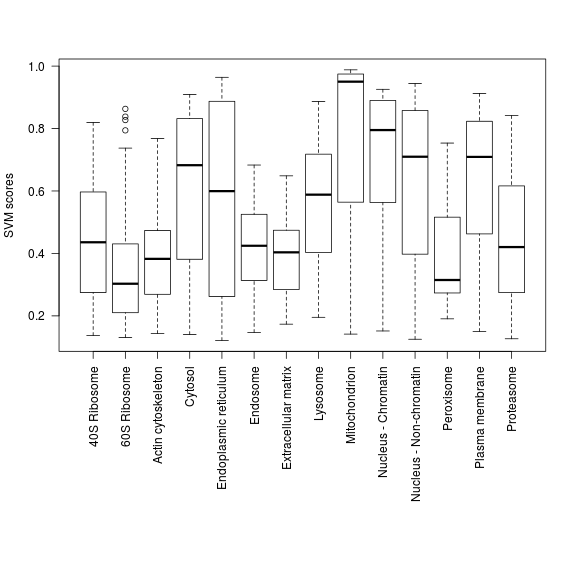
\includegraphics{figure/thresholds-1.png}
\caption{plot of chunk thresholds}
\end{figure}

There are many ways to set thresholds and the choice of method will
depend on the biological question and experimental design at hand. One
viable approach in the frame of the above experimetal design would be to
manually set a FDR, say 5\%, per organelle. To do this the user would
examine the top scoring predictions for each organelle, and then set a
threshold at the score at which they achieve 5\% of false assignments
per organelle. The definintion of a false assignment would depend on the
information available, for example, validity or lack of validity for the
localisation from another experiment as reported in the literature or a
reliable database. If such information is not available, one crude
method is to set a threshold per organelle by extracting the median or
3rd quantile score per organelle. For example, in the code chunk below,
we use the \texttt{orgQuants} function to extract the median organelle
scores and then pass these scores to the \texttt{getPrediction} function
to extract the new localisations that meet this scoring criteria. Any
sub-cellular predictions that fall below the specified thresholds are
labelled as unknown.

\begin{Shaded}
\begin{Highlighting}[]
\NormalTok{ts <-}\StringTok{ }\KeywordTok{orgQuants}\NormalTok{(hl, }
                \DataTypeTok{fcol =} \StringTok{"svm"}\NormalTok{, }
                \DataTypeTok{scol =} \StringTok{"svm.scores"}\NormalTok{,}
                \DataTypeTok{mcol =} \StringTok{"markers"}\NormalTok{, }
                \DataTypeTok{t =} \NormalTok{.}\DecValTok{5}\NormalTok{)}
\end{Highlighting}
\end{Shaded}

\begin{verbatim}
##            40S Ribosome            60S Ribosome      Actin cytoskeleton 
##               0.4356698               0.3028843               0.3825420 
##                 Cytosol   Endoplasmic reticulum                Endosome 
##               0.6825826               0.5995243               0.4245311 
##    Extracellular matrix                Lysosome           Mitochondrion 
##               0.4034908               0.5882168               0.9501241 
##     Nucleus - Chromatin Nucleus - Non-chromatin              Peroxisome 
##               0.7951459               0.7096694               0.3149301 
##         Plasma membrane              Proteasome 
##               0.7091667               0.4204304
\end{verbatim}

\begin{Shaded}
\begin{Highlighting}[]
\NormalTok{hl <-}\StringTok{ }\KeywordTok{getPredictions}\NormalTok{(hl,}
                     \DataTypeTok{fcol =} \StringTok{"svm"}\NormalTok{,}
                     \DataTypeTok{scol =} \StringTok{"svm.scores"}\NormalTok{, }
                     \DataTypeTok{mcol =} \StringTok{"markers"}\NormalTok{,}
                     \DataTypeTok{t =} \NormalTok{ts)}
\end{Highlighting}
\end{Shaded}

\begin{verbatim}
## ans
##            40S Ribosome            60S Ribosome      Actin cytoskeleton 
##                      86                     169                      86 
##                 Cytosol   Endoplasmic reticulum                Endosome 
##                     295                     479                      91 
##    Extracellular matrix                Lysosome           Mitochondrion 
##                      26                     125                     522 
##     Nucleus - Chromatin Nucleus - Non-chromatin              Peroxisome 
##                     230                     344                      38 
##         Plasma membrane              Proteasome                 unknown 
##                     325                     159                    2057
\end{verbatim}

The output of \texttt{getPredictons} is the original \texttt{MSnSet}
dataset with a new feature variable appended to the feature data called
\texttt{fcol.pred} (i.e.~in our case \texttt{svm.pred}) containing the
prediction results. The results can also be visualied using
\texttt{plot2D} function.

\begin{Shaded}
\begin{Highlighting}[]
\KeywordTok{dev.off}\NormalTok{()}
\end{Highlighting}
\end{Shaded}

\begin{verbatim}
## null device 
##           1
\end{verbatim}

\begin{Shaded}
\begin{Highlighting}[]
\KeywordTok{plot2D}\NormalTok{(hl, }\DataTypeTok{fcol =} \StringTok{"svm.pred"}\NormalTok{)}
\end{Highlighting}
\end{Shaded}

\begin{figure}[htbp]
\centering
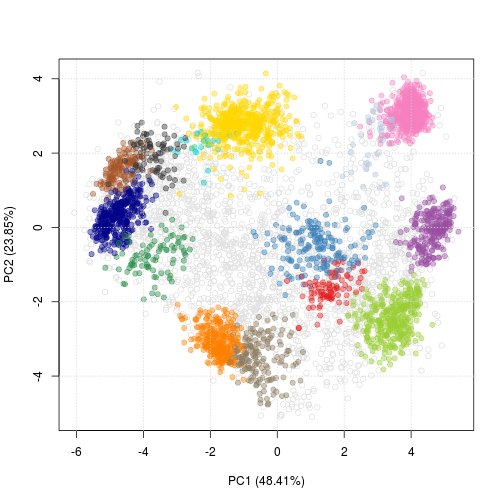
\includegraphics{figure/plotres-1.png}
\caption{plot of chunk plotres}
\end{figure}

There is also a dedicated interactive application to help users examine
these distributions in the
\emph{\href{http://bioconductor.org/packages/pRolocGUI}{pRolocGUI}}
package. This app can be launched via the \texttt{pRolocVis} function
and specifying the argument \texttt{app = "classify"} along with the
relevent \texttt{fcol}, \texttt{scol} and \texttt{mcol} which refer to
the columns in the feature data that contain the new assignments,
assignment scores and markers respectively (see also
\texttt{fvarLabels(svmres)}).

\begin{Shaded}
\begin{Highlighting}[]
\KeywordTok{library}\NormalTok{(}\StringTok{"pRolocGUI"}\NormalTok{)}
\KeywordTok{pRolocVis}\NormalTok{(hl, }
          \DataTypeTok{app =} \StringTok{"classify"}\NormalTok{,}
          \DataTypeTok{fcol =} \StringTok{"svm"}\NormalTok{,}
            \DataTypeTok{scol =} \StringTok{"svm.scores"}\NormalTok{,}
          \DataTypeTok{mcol =} \StringTok{"markers"}\NormalTok{)}
\end{Highlighting}
\end{Shaded}

\begin{figure}[htbp]
\centering
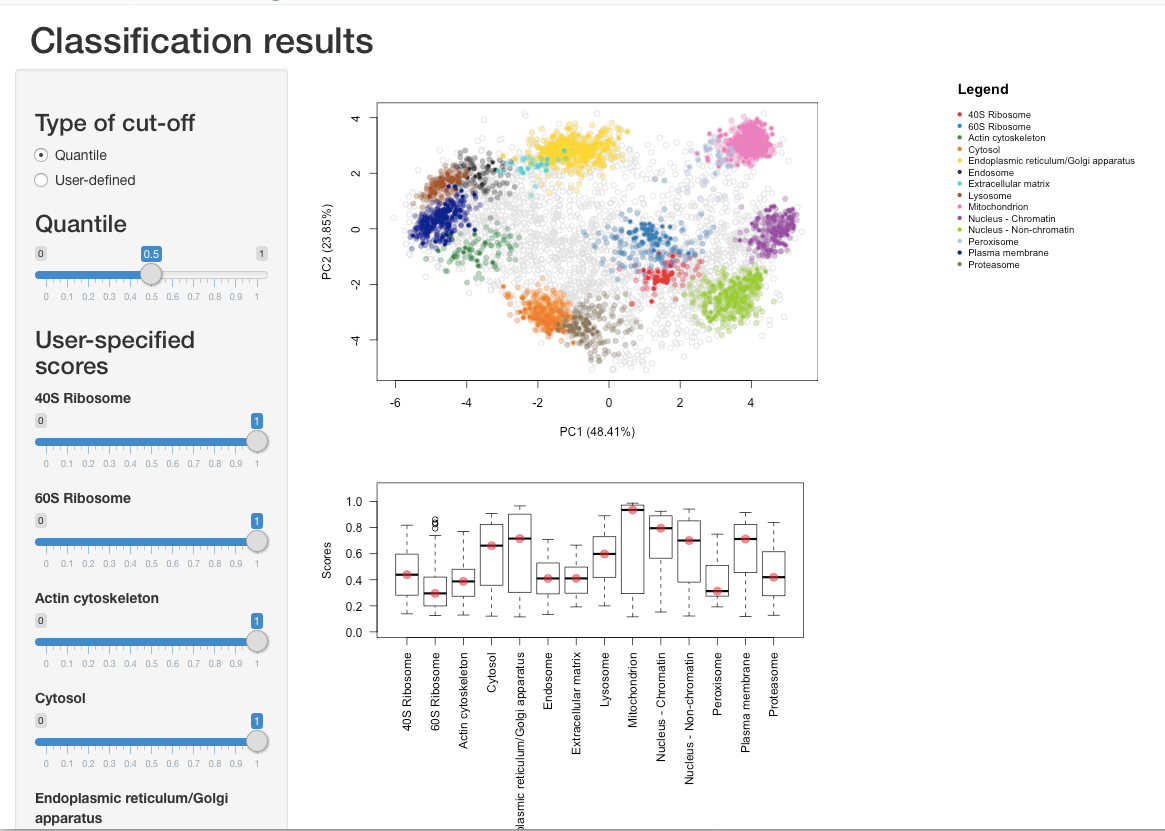
\includegraphics{./Figures/classify.png}
\caption{The classify application}
\end{figure}

The data is loaded and displayed on a PCA plot and a boxplot is used to
display the classifier scores by data class. On the left there is a
sidebar panel with sliders to control the thresholds upon which
classifications are made. There are two types of cut-off that the user
can choose from: (1) ``Quantile'' and (2) ``User-defined''. By default,
when the application is launched quatile scoring is selected and set to
0.5, the median. The class-specific score thresholds that correspond to
selecting the desired quantile are shown on as red dots on the boxplot.
The assignments on the PCA plot are also updated according to the
selected threshold. The quantile threshold can be set by moving the
corresponding quantile slider. If one wished to set their own cut-offs
the ``User-defined'' radio button must be selected and then the sliders
for defining user-specified scores become active and the scores and
highlighted on the boxplot by blue dots. For more information we refer
users to the
\emph{\href{http://bioconductor.org/packages/pRolocGUI}{pRolocGUI}}
tutorial
\href{http://bioconductor.org/packages/release/bioc/vignettes/pRolocGUI/inst/doc/pRolocGUI.html}{vignette}.

\subsection{Transfer learning}\label{transfer-learning}

In addition to high quality MS-based quantitative proteomics data there
exist a number of other sources of information that are freely available
in the public domain that may be useful to assign a protein to its
sub-cellular niche. For example, imaging from immunofluorescence
microscopy, protein annotations and sequences, and protein-protein
interactions among others, represent a rich and vast source of
complementary information. We can integrate this auxiliary information
with our primary MS-based quantitative data using a paradigm known as
transfer learning (TL). The integration of data between different
technologies is one of the biggest challenges in computational biology
to date and the
\emph{\href{http://bioconductor.org/packages/pRoloc}{pRoloc}} package
provides functionality to do such analyses. We recently developed two
transfer learning algorithms using a \emph{k}-NN and SVM framework and
applied them to the task of protein localisation prediction
{[}@Breckels:2016{]}. In this section we will begin with explaining the
concept of transfer learning and then show how to apply this in the
frame of spatial proteomics and protein localisation prediction.

In TL one typically has a primary task that they wish to solve, and some
complementary (often heterogeneous) auxiliary information that is
related to the primary learning objective, that can be used to help
solve the primary goal. For example, here our primary task is to assign
proteins to their sub-cellular niche with high generalisation accuracy
from data collected from quantitative MS-based experiments. In the
example below we extract Gene Ontology (GO) information to use as an
auxiliary data source to help solve our task of protein localisation
prediction.

Using the functions \texttt{setAnnotationParams} and \texttt{makeGoSet}
we can contruct an auxiliary \texttt{MSnSet} of GO terms, from the
primary data's features i.e.~the protein accession numbers. All the GO
terms associated to each accession number are retrieved and used to
create a binary matrix where a 1 (0) at position (i; j) indicates that
term j has (not) been used to annotate protein i. The GO terms are
retrieved from an appropriate repository using the
\emph{\href{http://bioconductor.org/packages/biomaRt}{biomaRt}} package.
The specific
\emph{\href{http://bioconductor.org/packages/Biomart}{Biomart}}
repository and query will depend on the species under study and the type
of identifiers. The first step is to construct the annotation parameters
that will enable to perform the query, this is done using
\texttt{setAnnotationParams}. Typing into the R console
\texttt{par \textless{}- setAnnotationParams()} will present two menus,
firstly asking you to identify the species of study, and then what type
of identifier you have used to annotate the proteins in your
\texttt{MSnSet}. It is also possible to pass patterns to match the
species e.g.~in the code chunk below we pass ``Mus musculus'', and the
identifier type for our data (see \texttt{featureNames(hl)}) which is
``Uniprot/Swissprot'', for the \texttt{Biocpkg("Biomart")} query.

\begin{Shaded}
\begin{Highlighting}[]
\NormalTok{par <-}\StringTok{ }\KeywordTok{setAnnotationParams}\NormalTok{(}\DataTypeTok{inputs =} \KeywordTok{c}\NormalTok{(}\StringTok{"Mus musculus"}\NormalTok{, }
                                      \StringTok{"UniProt/Swissprot"}\NormalTok{))}
\end{Highlighting}
\end{Shaded}

Now we have contructed the query parameters we can use the
\texttt{makeGoSet} function to retrieve and build an auxiliary GO
\texttt{MSnSet} as described above. By default, the cellular component
terms are downloaded, without any filtering on evidence codes. It is
also possible to download terms from the molecular function and
biological process GO namespaces, and also apply filtering based on
evidence codes as desired, see \texttt{?makeGoSet} for more details.

\begin{Shaded}
\begin{Highlighting}[]
\NormalTok{gocc <-}\StringTok{ }\KeywordTok{makeGoSet}\NormalTok{(hl, }\DataTypeTok{params =} \NormalTok{par, }
                  \DataTypeTok{namespace =} \StringTok{"cellular_component"}\NormalTok{, }
                  \DataTypeTok{evidence =} \OtherTok{NULL}\NormalTok{)}
\end{Highlighting}
\end{Shaded}

The function \texttt{makeGoSet} uses the
\emph{\href{http://bioconductor.org/packages/biomaRt}{biomaRt}} package
to query the relevent database (e.g.~Ensembl, Uniprot) for GO terms. All
GO terms that have been observed for the 5032 proteins in the hyperLOPIT
dataset are retieved. Users should note that the number of GO terms
retreived is also dependent on the database version queried and thus is
always subject to change. We find it is common to see many GO terms with
only one protein assigned to that term, these such terms generally do
not bring and information generally for building the classifier and thus
we can remove such GO terms by using the function
\texttt{filterBinMSnSet}.

\begin{Shaded}
\begin{Highlighting}[]
\NormalTok{gocc <-}\StringTok{ }\KeywordTok{filterBinMSnSet}\NormalTok{(hl)}
\end{Highlighting}
\end{Shaded}

Now we have generated our auxiliary data we can use the \emph{k}-NN
implementation of transfer learning available in
\texttt{Biocpkg("pRoloc")} to integrate this with our primary MS-based
quantitative proteomics data using the functions
\texttt{knntlOptimisation} to estimate the free-parameters for the
integration, and \texttt{knntlClassification} to do the predictions. We
have shown that using transfer learning in the context of spatial
proteomics results in the assignment of proteins to sub-cellular niches
with a higher generalisation accuracy than using standard supervised
machine learning with a single source of information
{[}@Breckels:2016{]}.

The first step, as with any machine learning algorithm, is to optimise
any free paramaters of the classifier. For the \emph{k}-NN TL classifier
there are two sets of parameters that need optimising: the first set are
the $k$'s for the primary and auxiliary data sources required for the
nearest neighbour calculations for each data source. The second set of
parameters (which is noted by a vector of $\theta$ weights) that require
optimising are the class weights, one per subcellular niche, that
control the proportion of primary and auxiliary data to use for
learning. A weight can take any real value number between 0 and 1. A
weight of $\theta = 1$ indicates that all weight is given to the primary
data (and this implicitly implies that a weight of $1 - \theta$ is given
to the auxiliary data, similarly a weight of $\theta = 0$ implies that
all weight is given to the auxiliary data (so 0 is given to the primary
source). If we conduct a parameter seach and test weights
$\theta = {0, 1/3, 2/3, 1}$ for each class, and if we have, for example
10 subcellular niches, this will result in \texttt{4\^{}10} different
combinations of parameters to test. The parameter optimisation is
therefore time consuming and as such we recommend you make use of a
computing cluster (code and submissing scripts are also available in the
supporting information). The markers in the \texttt{hl} dataset contain
14 subcellular classes. If we examine these markers and classes on the
PCA plot above we can see that in particular the two ribosomes and two
nuclear compartments are highly separated along the first two
components, this is also evident from the profiles plot which gives us a
good indication that these subcellular niches are well-resolved in the
hyperLOPIT dataset. Transfer learning is particularly useful for classes
that are not as well separated, we find that subcellular niches that are
well-separated under hyperLOPIT and LOPIT obtain a class score of 1
(i.e.~use only primary data from transfer learning
{[}@Breckels:2016{]}). Therefore, for the optimisation stage of the
analyses we can already infer a subcellular class weight of 1 for these
niches and only optimise over the remaining organelles. This can
signifciantly cut down optimisation time as by removing these 4 classes
from the optimisation (and not the classification) we only have
\texttt{4\^{}10} class weight combinations to consider instead of
\texttt{4\^{}14} combinations.

In the example below we remove these 4 classes from the marker set,
re-run the \texttt{knnOptimisation} for each data source and then run
the \texttt{knntlOptimisation} with the 10 remaining classes. (Note:
this is not run live as this the \texttt{hl} dataset with 10 classes,
707 markers and \texttt{4\^{}10} combinations of parameters takes
\textasciitilde{}76 hours to run on the University of Cambridge HPC
using 256 workers).

To remove the 4 classes and create a new column of markers in the
feature data called \texttt{tlmarkers} to use for the analysis:

\begin{Shaded}
\begin{Highlighting}[]
\NormalTok{## create new markers column for tl markers}
\KeywordTok{fData}\NormalTok{(hl)$tlmarkers <-}\StringTok{ }\KeywordTok{fData}\NormalTok{(hl)$markers}
\KeywordTok{fData}\NormalTok{(gocc)$tlmarkers <-}\StringTok{ }\KeywordTok{fData}\NormalTok{(gocc)$markers}

\NormalTok{## Remove 4 classes}
\NormalTok{torm  <-}\StringTok{ }\KeywordTok{c}\NormalTok{(}\StringTok{"40S Ribosome"}\NormalTok{, }\StringTok{"60S Ribosome"}\NormalTok{,}
           \StringTok{"Nucleus - Chromatin"}\NormalTok{, }
           \StringTok{"Nucleus - Non-chromatin"}\NormalTok{)}
\NormalTok{for (i in }\KeywordTok{seq}\NormalTok{(torm)) \{}
  \NormalTok{hl <-}\StringTok{ }\KeywordTok{fDataToUnknown}\NormalTok{(hl, }\DataTypeTok{from =} \NormalTok{torm[i], }\DataTypeTok{fcol =} \StringTok{"tlmarkers"}\NormalTok{)}
  \NormalTok{gocc <-}\StringTok{ }\KeywordTok{fDataToUnknown}\NormalTok{(gocc, }\DataTypeTok{from =} \NormalTok{torm[i], }\DataTypeTok{fcol =} \StringTok{"tlmarkers"}\NormalTok{)}
\NormalTok{\}}
\KeywordTok{getMarkerClasses}\NormalTok{(hl, }\DataTypeTok{fcol =} \StringTok{"tlmarkers"}\NormalTok{)}
\end{Highlighting}
\end{Shaded}

\begin{verbatim}
##  [1] "Actin cytoskeleton"    "Cytosol"              
##  [3] "Endoplasmic reticulum" "Endosome"             
##  [5] "Extracellular matrix"  "Lysosome"             
##  [7] "Mitochondrion"         "Peroxisome"           
##  [9] "Plasma membrane"       "Proteasome"
\end{verbatim}

\begin{Shaded}
\begin{Highlighting}[]
\KeywordTok{getMarkerClasses}\NormalTok{(gocc, }\DataTypeTok{fcol =} \StringTok{"tlmarkers"}\NormalTok{)}
\end{Highlighting}
\end{Shaded}

\begin{verbatim}
##  [1] "Actin cytoskeleton"    "Cytosol"              
##  [3] "Endoplasmic reticulum" "Endosome"             
##  [5] "Extracellular matrix"  "Lysosome"             
##  [7] "Mitochondrion"         "Peroxisome"           
##  [9] "Plasma membrane"       "Proteasome"
\end{verbatim}

Optimisation stage 1: run \texttt{knnOptimisation} to get the best $k$'s
for each data source.

\begin{Shaded}
\begin{Highlighting}[]
\NormalTok{## get best k's}
\NormalTok{kpopt <-}\StringTok{ }\KeywordTok{knnOptimisation}\NormalTok{(hl, }\DataTypeTok{fcol =} \StringTok{"tlmarkers"}\NormalTok{)}
\NormalTok{kaopt <-}\StringTok{ }\KeywordTok{knnOptimisation}\NormalTok{(gocc, }\DataTypeTok{fcol =} \StringTok{"tlmarkers"}\NormalTok{)}
\KeywordTok{plot}\NormalTok{(kpopt)}
\KeywordTok{plot}\NormalTok{(kaopt)}
\end{Highlighting}
\end{Shaded}

From examining the parameter seach plots we find the best $k$'s for both
the primary and auxiliary are 3.

Optimisation stage 2: run \texttt{knntlOptimisation} to get the best
transfer learning weights for each sub-cellular class.

\begin{Shaded}
\begin{Highlighting}[]
\NormalTok{## Set appropriate parallelisation backend and  }
\NormalTok{## number of workers for the tl}
\NormalTok{par <-}\StringTok{ }\KeywordTok{SnowParam}\NormalTok{(255L, }\DataTypeTok{type =} \StringTok{"MPI"}\NormalTok{)}

\NormalTok{## Now peform tl optimisation }
\NormalTok{tlopt <-}\StringTok{ }\KeywordTok{knntlOptimisation}\NormalTok{(hl, gocc,}
                           \DataTypeTok{fcol =} \StringTok{"tlmarkers"}\NormalTok{,}
                           \DataTypeTok{length.out =} \DecValTok{4}\NormalTok{, }
                           \DataTypeTok{times =} \DecValTok{50}\NormalTok{,}
                           \DataTypeTok{xval =} \DecValTok{5}\NormalTok{, }\DataTypeTok{k =} \KeywordTok{c}\NormalTok{(}\DecValTok{3}\NormalTok{, }\DecValTok{3}\NormalTok{),}
                           \DataTypeTok{BPPARAM =} \NormalTok{par}
  \NormalTok{)}
\end{Highlighting}
\end{Shaded}

The results of the optimisation can be visalised using the \texttt{plot}
method for \texttt{"ThetaRegRes"} objects:

\begin{Shaded}
\begin{Highlighting}[]
\KeywordTok{plot}\NormalTok{(tlopt)}
\end{Highlighting}
\end{Shaded}

\begin{figure}[htbp]
\centering
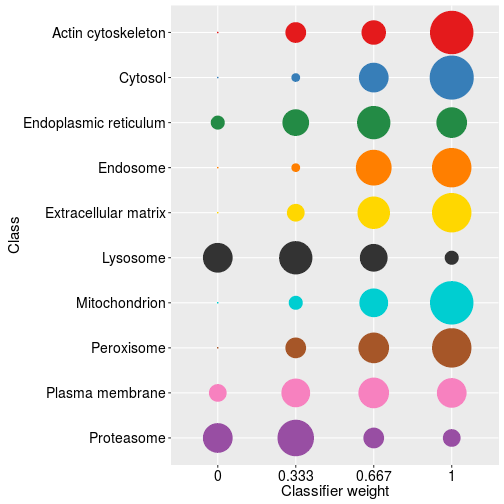
\includegraphics{figure/plottl-1.png}
\caption{plot of chunk plottl}
\end{figure}

Looking at the bubble plot displaying the distribution of best weights
over the 50 runs we find that for many of the subcellular niches a
weight of 1 is most popular (i.e.~use only primary hyperLOPIT data in
classification), this is unsuprising as we already know the dataset is
well resolved for these classes. We see that the most popular weights
for the proteasome and lysosome tend to be towards 0, indicating that
these niches are well-resolved in the Gene Ontology. This tells us that
we would benefit from including auxiliary GO information in our
classifier for these subcellular compartments. The plasma membrane
weights are relatively equally spread between using hyperLOPIT and GO
data. Using the \texttt{getParams} function we can return the best
weights and then use this as input for the classification.

One of the benefits of the algorithm is the ability to manually select
weights for each class. In the optimisation above, for time constraints,
we removed the two ribosomal subunits and the two nulcear compartments,
and therefore in the code chunk below when we extract the best
parameters, these subcellular niches are not included. To include these
4 subcellular niches in the next classification step we must include
them in the parameters so we infer a weight of 1 for each of these
niches as we know they are well resolved in hyperLOPIT. We then re-order
the weights according to \texttt{getMarkerClasses} and perform the
classification using the function \texttt{knntlClassification}.

\begin{Shaded}
\begin{Highlighting}[]
\NormalTok{## best parameters for the 10 classes}
\NormalTok{(bestpar <-}\StringTok{ }\KeywordTok{getParams}\NormalTok{(tlopt))}
\end{Highlighting}
\end{Shaded}

\begin{verbatim}
##    Actin cytoskeleton               Cytosol Endoplasmic reticulum 
##             1.0000000             1.0000000             0.6666667 
##              Endosome  Extracellular matrix              Lysosome 
##             1.0000000             1.0000000             0.3333333 
##         Mitochondrion            Peroxisome       Plasma membrane 
##             1.0000000             1.0000000             0.6666667 
##            Proteasome 
##             0.3333333
\end{verbatim}

\begin{Shaded}
\begin{Highlighting}[]
\NormalTok{## add weights for classes not included in the optimisation}
\NormalTok{otherweights <-}\StringTok{ }\KeywordTok{rep}\NormalTok{(}\DecValTok{1}\NormalTok{, }\DecValTok{4}\NormalTok{)}
\KeywordTok{names}\NormalTok{(otherweights) <-}\StringTok{ }\KeywordTok{c}\NormalTok{(}\StringTok{"40S Ribosome"}\NormalTok{, }\StringTok{"60S Ribosome"}\NormalTok{, }
                         \StringTok{"Nucleus - Chromatin"}\NormalTok{, }
                         \StringTok{"Nucleus - Non-chromatin"}\NormalTok{)}
\NormalTok{(bestpar <-}\StringTok{ }\KeywordTok{c}\NormalTok{(bestpar, otherweights))}
\end{Highlighting}
\end{Shaded}

\begin{verbatim}
##      Actin cytoskeleton                 Cytosol   Endoplasmic reticulum 
##               1.0000000               1.0000000               0.6666667 
##                Endosome    Extracellular matrix                Lysosome 
##               1.0000000               1.0000000               0.3333333 
##           Mitochondrion              Peroxisome         Plasma membrane 
##               1.0000000               1.0000000               0.6666667 
##              Proteasome            40S Ribosome            60S Ribosome 
##               0.3333333               1.0000000               1.0000000 
##     Nucleus - Chromatin Nucleus - Non-chromatin 
##               1.0000000               1.0000000
\end{verbatim}

\begin{Shaded}
\begin{Highlighting}[]
\NormalTok{## re-order classes }
\NormalTok{bestpar <-}\StringTok{ }\NormalTok{bestpar[}\KeywordTok{getMarkerClasses}\NormalTok{(hl)]}

\NormalTok{## Do the classification}
\NormalTok{hl <-}\StringTok{ }\KeywordTok{knntlClassification}\NormalTok{(hl, gocc, }\DataTypeTok{bestTheta =} \NormalTok{bestpar, }
                          \DataTypeTok{k =} \KeywordTok{c}\NormalTok{(}\DecValTok{3}\NormalTok{, }\DecValTok{3}\NormalTok{))}
\end{Highlighting}
\end{Shaded}

The results from the classification results and associated scores are
appended to the \texttt{fData} slot and named \texttt{knntl} and
\texttt{knntl.scores} respectively. Results can be visualised using
\texttt{plot2D}, scores assessed and cutoffs calculated using the
\texttt{classify} app in \texttt{pRolocVis}, predictions obtained using
\texttt{getPredictions} in the same way as demonstrated above for the
SVM classifier.

\subsection{Unsupervised machine
learning}\label{unsupervised-machine-learning}

In \texttt{pRoloc} there is functionality for unsupervsied machine
learning methods. In unsupervised learning, the training data consists
of a set of input vectors e.g.~protein profiles, for which we do not
have information about the class label e.g.~localisation. The main goal
in unsupervised learning is to uncover groups of similar examples within
the data, this is termed clustering. Ordinance methods such as principal
components analysis (PCA) also fall into the category of unsupervised
learning methods, where the data can be projected from a
high-dimensional spcae down to two or three dimensions for the purpose
of visualisation.

As described and demonstrated already above, PCA is a valuable and
powerful method for data visualisation and quality control. We do not do
any unsupervised clustering in the frame of the above spatial proteomics
workflow as although clustering can be useful for grouping labelled data
into categories e.g.~see the \texttt{mrkHClust} function, we do not find
it adaquete for spatial proteomics data analysis. We find supervised
learning more suited to the task of protein localisation prediction in
which we use high-quality curated marker proteins to build a classifier,
instead of using an entirely unsupervised approach to look for clusters
and then look for enrichment of organelles and complexes. In the latter
we do not make good use of valuable prior knowledge, and in our
experience unsupervised clustering can be extremely difficult due poor
estimates of the number of clusters that may appear in the data.

\section{Writing and exporting data}\label{writing-and-exporting-data}

A \texttt{MSnSet} can be exported from R using the \texttt{write.exprs}
function. This function writes the expression values to a tab (the
defualt, or other type e.g.e.g.~comma, as specified in
\texttt{write,table}) separated file. There argument \texttt{fDataCols}
can be used to specify which \texttt{featureData} columns (as column
names, column number or \texttt{logical}) to append to the right of the
expression matrix.

In the below code chunk we write the \texttt{hl} object to a csv file.
The \texttt{file} argument is used to specify the file path, the
\texttt{sep} argument specifies the field separator string, here we use
a comma, finally as we want to write all the information in the
\texttt{featureData} to the file, as well as the expression data, we
specify \texttt{fDataCols = 1:ncol(hl)} i.e.~write everything in the
\texttt{featureData} to the file \texttt{"hl.csv"}.

\begin{Shaded}
\begin{Highlighting}[]
\KeywordTok{write.exprs}\NormalTok{(hl, }\DataTypeTok{file =} \StringTok{"hl.csv"}\NormalTok{, }\DataTypeTok{sep =} \StringTok{","}\NormalTok{, }
            \DataTypeTok{fDataCols =} \DecValTok{1}\NormalTok{:}\KeywordTok{ncol}\NormalTok{(hl))}
\end{Highlighting}
\end{Shaded}

Individual R objects, such a parameters from the machine learning
optimisations, can be save using the standard \texttt{save} function in
R. For example, to save and then re-load the parameters from the SVM
optimisation,

\begin{Shaded}
\begin{Highlighting}[]
\NormalTok{## To save the parameters as an R object}
\KeywordTok{save}\NormalTok{(params, }\DataTypeTok{file =} \StringTok{"svmparams.rda"}\NormalTok{)}

\NormalTok{## To re-load after saving}
\KeywordTok{load}\NormalTok{(}\DataTypeTok{file =} \StringTok{"svmparams.rda"}\NormalTok{)}
\end{Highlighting}
\end{Shaded}

\section{Session information}\label{session-information}

The function \texttt{sessionInfo} provides a summary of all packages and
versions used to generate this document. This enables us to record the
exact state of our session that lead to these exact results. Conversely,
if the script stops working of if it returns different results, we are
in a position to re-generate the original results using the adequate
software versions and retrace changes in the software that lead to
failure and/or different results.

\begin{Shaded}
\begin{Highlighting}[]
\KeywordTok{sessionInfo}\NormalTok{()}
\end{Highlighting}
\end{Shaded}

\begin{verbatim}
## R version 3.3.1 Patched (2016-08-02 r71022)
## Platform: x86_64-pc-linux-gnu (64-bit)
## Running under: Ubuntu 14.04.5 LTS
## 
## locale:
##  [1] LC_CTYPE=en_GB.UTF-8       LC_NUMERIC=C              
##  [3] LC_TIME=en_GB.UTF-8        LC_COLLATE=en_GB.UTF-8    
##  [5] LC_MONETARY=en_GB.UTF-8    LC_MESSAGES=en_GB.UTF-8   
##  [7] LC_PAPER=en_GB.UTF-8       LC_NAME=C                 
##  [9] LC_ADDRESS=C               LC_TELEPHONE=C            
## [11] LC_MEASUREMENT=en_GB.UTF-8 LC_IDENTIFICATION=C       
## 
## attached base packages:
## [1] stats4    parallel  methods   stats     graphics  grDevices utils    
## [8] datasets  base     
## 
## other attached packages:
##  [1] pRolocdata_1.11.9    pRoloc_1.13.15       MLInterfaces_1.53.1 
##  [4] cluster_2.0.4        annotate_1.51.1      XML_3.98-1.4        
##  [7] AnnotationDbi_1.35.4 IRanges_2.7.15       S4Vectors_0.11.17   
## [10] MSnbase_1.99.2       ProtGenerics_1.5.1   BiocParallel_1.7.8  
## [13] mzR_2.7.6            Rcpp_0.12.7          Biobase_2.33.3      
## [16] BiocGenerics_0.19.2  gridExtra_2.2.1      BiocStyle_2.1.32    
## [19] knitr_1.14          
## 
## loaded via a namespace (and not attached):
##  [1] minqa_1.2.4           colorspace_1.2-6      hwriter_1.3.2        
##  [4] class_7.3-14          modeltools_0.2-21     mclust_5.2           
##  [7] pls_2.5-0             base64enc_0.1-3       proxy_0.4-16         
## [10] MatrixModels_0.4-1    affyio_1.43.0         flexmix_2.3-13       
## [13] mvtnorm_1.0-5         codetools_0.2-14      splines_3.3.1        
## [16] doParallel_1.0.10     impute_1.47.0         robustbase_0.92-6    
## [19] jsonlite_1.1          nloptr_1.0.4          caret_6.0-71         
## [22] pbkrtest_0.4-6        rda_1.0.2-2           kernlab_0.9-24       
## [25] vsn_3.41.0            sfsmisc_1.1-0         shiny_0.14           
## [28] sampling_2.7          assertthat_0.1        Matrix_1.2-7.1       
## [31] limma_3.29.21         formatR_1.4           htmltools_0.3.5      
## [34] quantreg_5.29         tools_3.3.1           ggvis_0.4.3          
## [37] gtable_0.2.0          affy_1.51.1           reshape2_1.4.1       
## [40] dplyr_0.5.0           MALDIquant_1.15       trimcluster_0.1-2    
## [43] gdata_2.17.0          preprocessCore_1.35.0 nlme_3.1-128         
## [46] iterators_1.0.8       fpc_2.1-10            stringr_1.1.0        
## [49] lme4_1.1-12           lpSolve_5.6.13        mime_0.5             
## [52] gtools_3.5.0          dendextend_1.3.0      DEoptimR_1.0-6       
## [55] zlibbioc_1.19.0       MASS_7.3-45           scales_0.4.0         
## [58] BiocInstaller_1.23.9  pcaMethods_1.65.0     SparseM_1.72         
## [61] RColorBrewer_1.1-2    ggplot2_2.1.0         biomaRt_2.29.2       
## [64] rpart_4.1-10          stringi_1.1.1         RSQLite_1.0.0        
## [67] genefilter_1.55.2     randomForest_4.6-12   foreach_1.4.3        
## [70] e1071_1.6-7           prabclus_2.2-6        bitops_1.0-6         
## [73] mzID_1.11.2           evaluate_0.9          lattice_0.20-34      
## [76] htmlwidgets_0.7       gbm_2.1.1             plyr_1.8.4           
## [79] magrittr_1.5          R6_2.1.3              DBI_0.5-1            
## [82] whisker_0.3-2         mgcv_1.8-15           survival_2.39-5      
## [85] RCurl_1.95-4.8        nnet_7.3-12           tibble_1.2           
## [88] msdata_0.12.1         car_2.1-3             mlbench_2.1-1        
## [91] grid_3.3.1            FNN_1.1               threejs_0.2.2        
## [94] digest_0.6.10         diptest_0.75-7        xtable_1.8-2         
## [97] httpuv_1.3.3          munsell_0.4.3
\end{verbatim}

It is always important to include session information details along with
a \href{http://adv-r.had.co.nz/Reproducibility.html}{short reproducible
example} highlighting the problem or
\href{https://support.bioconductor.org/}{question} at hand.
